\documentclass[12pt,dvipdfmx]{beamer}
\usepackage{graphicx}
\DeclareGraphicsExtensions{.pdf}
\DeclareGraphicsExtensions{.eps}
\graphicspath{{out/tex/svg/}}
\usepackage{listings}
\usepackage{fancybox}
\usepackage{hyperref}
\usepackage{color}

\newcommand{\plusequal}{\mbox{\tt\ += }}
\newcommand{\minusequal}{\mbox{\tt\ -= }}
\newcommand{\divequal}{\mbox{\tt\ /= }}
\newcommand{\plusplus}{\mbox{\tt\ ++ }}

%% OpenMP section numbers
\newcommand{\sectionompparallel}{{\href{https://www.openmp.org/spec-html/5.0/openmpse14.html\#x54-800002.6}{2.6}}}
\newcommand{\sectionompdeterminenumthreads}{{\href{https://www.openmp.org/spec-html/5.0/openmpsu35.html\#x55-880002.6.1}{2.6.1}}}
\newcommand{\sectionompfor}{{\href{https://www.openmp.org/spec-html/5.0/openmpsu41.html\#x64-1290002.9.2}{2.9.2}}}
\newcommand{\sectionompsimd}{{\href{https://www.openmp.org/spec-html/5.0/openmpsu42.html\#x65-1390002.9.3}{2.9.3}}}
\newcommand{\sectionompdeclaresimd}{{\href{https://www.openmp.org/spec-html/5.0/openmpsu42.html\#x65-1390002.9.3.3}{2.9.3.3}}}
\newcommand{\sectionompforform}{{\href{https://www.openmp.org/spec-html/5.0/openmpsu40.html\#x63-1260002.9.1}{2.9.1}}}
\newcommand{\sectionomptask}{{\href{https://www.openmp.org/spec-html/5.0/openmpsu46.html\#x70-2000002.10.1}{2.10.1}}}
\newcommand{\sectionomptaskwait}{{\href{https://www.openmp.org/spec-html/5.0/openmpsu93.html\#x124-4690002.17.5}{2.17.5}}}
\newcommand{\sectionompdataenv}{{\href{https://www.openmp.org/spec-html/5.0/openmpse27.html\#x135-5430002.19}{2.19}}}
\newcommand{\sectionompreduction}{{\href{https://www.openmp.org/spec-html/5.0/openmpsu107.html\#x140-5800002.19.5}{2.19.5}}}
\newcommand{\sectionompdeclarereduction}{{\href{https://www.openmp.org/spec-html/5.0/openmpsu107.html\#x140-5800002.19.5}{2.19.5.7}}}
\newcommand{\sectionompgetnumthreads}{{\href{https://www.openmp.org/spec-html/5.0/openmpsu111.html\#x148-6450003.2.2}{3.2.2}}}
\newcommand{\sectionompgetmaxthreads}{{\href{https://www.openmp.org/spec-html/5.0/openmpsu112.html\#x149-6510003.2.3}{3.2.3}}}
\newcommand{\sectionompgetthreadnum}{{\href{https://www.openmp.org/spec-html/5.0/openmpsu113.html\#x150-6570003.2.4}{3.2.4}}}



%%%%%%%%%%%%%%%%%%%%%%%%%%%
%%% themes
%%%%%%%%%%%%%%%%%%%%%%%%%%%
%\usetheme{Szeged} 
\usetheme{Madrid}

%% no navigation bar
% default boxes Bergen Boadilla Madrid Pittsburgh Rochester
%% tree-like navigation bar
% Antibes JuanLesPins Montpellier
%% toc sidebar
% Berkeley PaloAlto Goettingen Marburg Hannover Berlin Ilmenau Dresden Darmstadt Frankfurt Singapore Szeged
%% Section and Subsection Tables
% Copenhagen Luebeck Malmoe Warsaw

%%%%%%%%%%%%%%%%%%%%%%%%%%%
%%% innerthemes
%%%%%%%%%%%%%%%%%%%%%%%%%%%
% \useinnertheme{circles}	% default circles rectangles rounded inmargin

%%%%%%%%%%%%%%%%%%%%%%%%%%%
%%% outerthemes
%%%%%%%%%%%%%%%%%%%%%%%%%%%
% outertheme
% \useoutertheme{default}	% default infolines miniframes smoothbars sidebar sprit shadow tree smoothtree


%%%%%%%%%%%%%%%%%%%%%%%%%%%
%%% colorthemes
%%%%%%%%%%%%%%%%%%%%%%%%%%%
\usecolortheme{seahorse}
%% special purpose
% default structure sidebartab 
%% complete 
% albatross beetle crane dove fly seagull 
%% inner
% lily orchid rose
%% outer
% whale seahorse dolphin

%%%%%%%%%%%%%%%%%%%%%%%%%%%
%%% fontthemes
%%%%%%%%%%%%%%%%%%%%%%%%%%%
\usefonttheme{serif}  
% default professionalfonts serif structurebold structureitalicserif structuresmallcapsserif

%%%%%%%%%%%%%%%%%%%%%%%%%%%
%%% generally useful beamer settings
%%%%%%%%%%%%%%%%%%%%%%%%%%%
% 
\AtBeginDvi{\special{pdf:tounicode EUC-UCS2}}
% do not show navigation
\setbeamertemplate{navigation symbols}{}
% show page numbers
\setbeamertemplate{footline}[frame number]


%%%%%%%%%%%%%%%%%%%%%%%%%%%
%%% define some colors for convenience
%%%%%%%%%%%%%%%%%%%%%%%%%%%

\newcommand{\mido}[1]{{\color{green}#1}}
\newcommand{\mura}[1]{{\color{purple}#1}}
\newcommand{\ore}[1]{{\color{orange}#1}}
\newcommand{\ao}[1]{{\color{blue}#1}}
\newcommand{\aka}[1]{{\color{red}#1}}

\setbeamercolor{ex}{bg=cyan!20!white}

%%%%%%%%%%%%%%%%%%%%%%%%%%%
%%% how to typset code
%%%%%%%%%%%%%%%%%%%%%%%%%%%

\lstset{language = C,
numbers = left,
numberstyle = {\tiny \emph},
numbersep = 10pt,
breaklines = true,
breakindent = 40pt,
frame = tlRB,
frameround = ffft,
framesep = 3pt,
rulesep = 1pt,
rulecolor = {\color{blue}},
rulesepcolor = {\color{blue}},
flexiblecolumns = true,
keepspaces = true,
basicstyle = \ttfamily\scriptsize,
identifierstyle = ,
commentstyle = \it\scriptsize,
stringstyle = ,
showstringspaces = false,
tabsize = 4,
escapechar=\@,
}

\title{OpenMP}
\institute{}
\author{Kenjiro Taura}
\date{}

\AtBeginSection[] % Do nothing for \section*
{
\begin{frame}
\frametitle{Contents}
\tableofcontents[currentsection,currentsubsection]
\end{frame}
}

\AtBeginSubsection[] % Do nothing for \section*
{
\begin{frame}
\frametitle{Contents}
\tableofcontents[currentsection,currentsubsection]
\end{frame}
}

\begin{document}
\maketitle

%%%%%%%%%%%%%%%%%%%%%%%%%%%%%%%%%% 
\begin{frame}
\frametitle{Contents}
\tableofcontents
\end{frame}


\iffalse
%=================================
\section{Overview}
%=================================

%%%%%%%%%%%%%%%%% 
\begin{frame}
\frametitle{Goal}
\begin{itemize}
\item learn OpenMP, by far the most widespread standard API
  for shared memory parallel programming
%\item learn how it differs from TBB
\item learn that various schedulers execute your
  parallel programs differently
\end{itemize}
\end{frame}
\fi

\section{A Running Example: SpMV}
%%%%%%%%%%%%%%%%%
\begin{frame}
  \frametitle{A running example: Sparse Matrix Vector Multiply (SpMV)}
  \begin{itemize}
  \item sparse matrix : a matrix whose elements are mostly zeros
  \item i.e. the number of non-zero elements (nnz) $\ll$ the number of all elements ($M \times N$)
    \begin{itemize}
    \item $M$ : the number of rows
    \item $N$ : the number of columns
    \end{itemize}
  \end{itemize}

  \begin{center}
  
\includegraphics[width=0.4\textwidth]{out/pdf/svg/spmv.pdf}
  \end{center}
\end{frame}

%%%%%%%%%%%%%%%%% 
\begin{frame}
  \frametitle{Sparse matrices appear everywhere}
  \begin{itemize}
  \item \ao{meshes} in scientific simulation
    \begin{itemize}
    \item $A_{i,j} = $ a weight connecting nodes $i$ and $j$ in the mesh
    \end{itemize}

  \item \ao{graphs}, which in turn appear in many applications
    \begin{itemize}
    \item $A_{i,j} = $ the weight of the edge $i \rightarrow j$ (or $j \rightarrow i$)
    \item Web, social network, road/traffic networks,
      metabolic pathways, etc.
    \end{itemize}
    
  \item many problems can be solved using SpMV
    \begin{itemize}
    \item eigenvalues (including PageRank, graph partitioning, etc.)
    \item partial differential equation
    \item \ldots
    \end{itemize}
  \end{itemize}
\end{frame}

%%%%%%%%%%%%%%%%% 
\begin{frame}
  \frametitle{What makes ``sparse''
    matrix different from ordinary (dense) matrix?}

  \begin{itemize}
  \item the number of non-zero elements are so small that
    representing it as $M \times N$ array is too wasteful
    (or just impossible)
  \item $\rightarrow$ use a data structure that takes memory/computation
    only (or mostly) for non-zero elements
    (coordinate list, compressed sparse row, etc.)
  \item []
      \begin{center}
        
\includegraphics[width=0.3\textwidth]{out/pdf/svg/spmv.pdf}
      \end{center}
  \end{itemize}

\end{frame}

%%%%%%%%%%%%%%%%% 
\begin{frame}[fragile]
  \frametitle{Coordinate list (COO)}
  \begin{columns}
    \begin{column}{0.5\textwidth}
  \begin{itemize}
  \item represent a matrix as a list of $(i, j, A_{i,j})$'s
  \item data format:
\begin{lstlisting}
struct coo {
  int n_rows, n_cols, nnz;
  /* nnz elements */
  struct { i, j, Aij } * elems;
};
\end{lstlisting}
\item SpMV ($y = Ax$)
\begin{lstlisting}
for (k = 0; k < A.nnz; k++) {
  i,j,Aij = A.elems[k];
  y[i] += Aij * x[j];
}
\end{lstlisting}
\end{itemize}
    \end{column}
    \begin{column}{0.5\textwidth}
      \begin{center}
        
\includegraphics[width=0.9\textwidth]{out/pdf/svg/spmv_coo.pdf}
      \end{center}
    \end{column}
  \end{columns}
\end{frame}


%%%%%%%%%%%%%%%%% 
\begin{frame}[fragile]
  \frametitle{Compressed sparse row (CSR)}
  \begin{itemize}
  \item puts elements of a single row in a contiguous range 
  \item an index (number) specifies where a particular row begins
    in the {\tt elems} array
  \item $\rightarrow$ no need to have $i$ for every single element
  \item data format:
\begin{lstlisting}
struct coo {
  int n_rows, n_cols, nnz;    
  struct { j, Aij } * elems; // nnz elements
  int * row_start; // n_rows elements
};
\end{lstlisting}
{\tt elems[row\_start[$i$]]} $\cdots$ {\tt elems[row\_start[$i+1$]]}
are the elements in the $i$th row
\item SpMV ($y = Ax$)
\begin{lstlisting}
for (i = 0; i < A.n_rows; i++) {
  for (k = A.row_start[i]; k < A.row_start[i+1]; k++) {
    j,Aij = A.elems[k];
    y[i] += Aij * x[j];
  } }
\end{lstlisting}
\end{itemize}
\end{frame}


%%%%%%%%%%%%%%%%% 
\begin{frame}
\frametitle{OpenMP}
\begin{itemize}
\item {\em de fact\/} standard model for programming shared memory machines
\item C/C++/Fortran + \ao{directives + APIs}
  \begin{itemize}
  \item by \ao{\tt \#pragma} in C/C++
  \item by comments in Fortran
  \end{itemize}
\item many free/vendor compilers, including GCC,
  \href{https://llvm.org/}{LLVM},
  \href{https://docs.nvidia.com/hpc-sdk/index.html}{NVIDIA HPC SDK}
\end{itemize}
\end{frame}


%%%%%%%%%%%%%%%%% 
\begin{frame}
\frametitle{OpenMP reference}
\begin{itemize}
\item official home page:
  \url{http://openmp.org/}
\item specification:
  \url{http://openmp.org/wp/openmp-specifications/}
\item latest version is 5.0
(\url{https://www.openmp.org/spec-html/5.0/openmp.html})
\item section numbers below refer to those in OpenMP spec 5.0
\end{itemize}

\end{frame}

\iffalse
%%%%%%%%%%%%%%%%% 
\begin{frame}
\frametitle{GCC and OpenMP}
\begin{itemize}
\item see \url{http://gcc.gnu.org/wiki/openmp} for details
\item gcc 4.2 $\rightarrow$ OpenMP spec 2.5
\item gcc 4.4 $\rightarrow$ OpenMP spec 3.0 (task parallelism)
\item gcc 4.7 $\rightarrow$ OpenMP spec 3.1
\item gcc 4.9 $\rightarrow$ OpenMP spec 4.0 (SIMD)
\item gcc 9 $\rightarrow$ initial OpenMP 5 support
\end{itemize}
\end{frame}

%%%%%%%%%%%%%%%%% 
\begin{frame}[fragile]
\frametitle{Compiling/running OpenMP programs with GCC}

\begin{itemize}
\item compile with {\tt -fopenmp}
\begin{lstlisting}
$ gcc -Wall @\ao{\tt -fopenmp}@ program.c
\end{lstlisting}
%$
\item run the executable specifying the number of threads
with {\tt OMP\_NUM\_THREADS} environment variable
\begin{lstlisting}
$ @\ao{\tt OMP\_NUM\_THREADS=1}@ ./a.out  # use 1 thread
$ @\ao{\tt OMP\_NUM\_THREADS=4}@ ./a.out  # use 4 threads
\end{lstlisting}

\item see \sectionompdeterminenumthreads\
``Determining the Number of Threads for a parallel Region''
for other ways to control the number of threads
\end{itemize}
\end{frame}
\fi

%%%%%%%%%%%%%%%%% 
\begin{frame}[fragile]
\frametitle{Compiling OpenMP programs for multicores}
\begin{itemize}
\item GCC and LLVM ({\tt clang/clang++}) : compile with {\tt -fopenmp}
\begin{lstlisting}
$ clang -Wall @\ao{\tt -fopenmp}@ program.c
$ gcc -Wall @\ao{\tt -fopenmp}@ program.c
\end{lstlisting}

\item NVIDIA HPC SDK ({\tt nvc/nvc++}) : compile with {\tt -mp}
\begin{lstlisting}
$ nvc -Wall @\ao{\tt -mp}@ program.c
\end{lstlisting}
% $
\item In this lecture, we use LLVM and NVIDIA HPC SDK,
  as they support OpenMP for multicore, GPU offloading,
  and CUDA
\end{itemize}
\end{frame}

%%%%%%%%%%%%%%%%% 
\begin{frame}[fragile]
\frametitle{Running OpenMP programs}
\begin{itemize}
\item run the executable specifying the number of threads
with {\tt OMP\_NUM\_THREADS} environment variable
\begin{lstlisting}
$ @\ao{\tt OMP\_NUM\_THREADS=1}@ ./a.out  # use 1 thread
$ @\ao{\tt OMP\_NUM\_THREADS=4}@ ./a.out  # use 4 threads
\end{lstlisting}

\item if {\tt OMP\_NUM\_THREADS} is unspecified,
  it uses the number of available
  processors visible to OS, including hyperthreading

\item see \sectionompdeterminenumthreads\
``Determining the Number of Threads for a parallel Region''
for more details and other ways to control the number of threads
\end{itemize}
\end{frame}

%=================================
\section{{\tt parallel} pragma}
%=================================

%%%%%%%%%%%%%%%%% 
\begin{frame}
\frametitle{Two pragmas you must know first}
\begin{columns}
\begin{column}{0.5\textwidth}
\begin{itemize}

\item \ao{\tt \#pragma omp parallel} 
to launch a team of threads (\sectionompparallel)
\item then \ao{\tt \#pragma omp for} to distribute 
iterations to threads (\sectionompfor)
\end{itemize}
Note: all OpenMP pragmas have the common format: 
{\tt \#pragma omp \ldots}
\end{column}
\begin{column}{0.5\textwidth}
%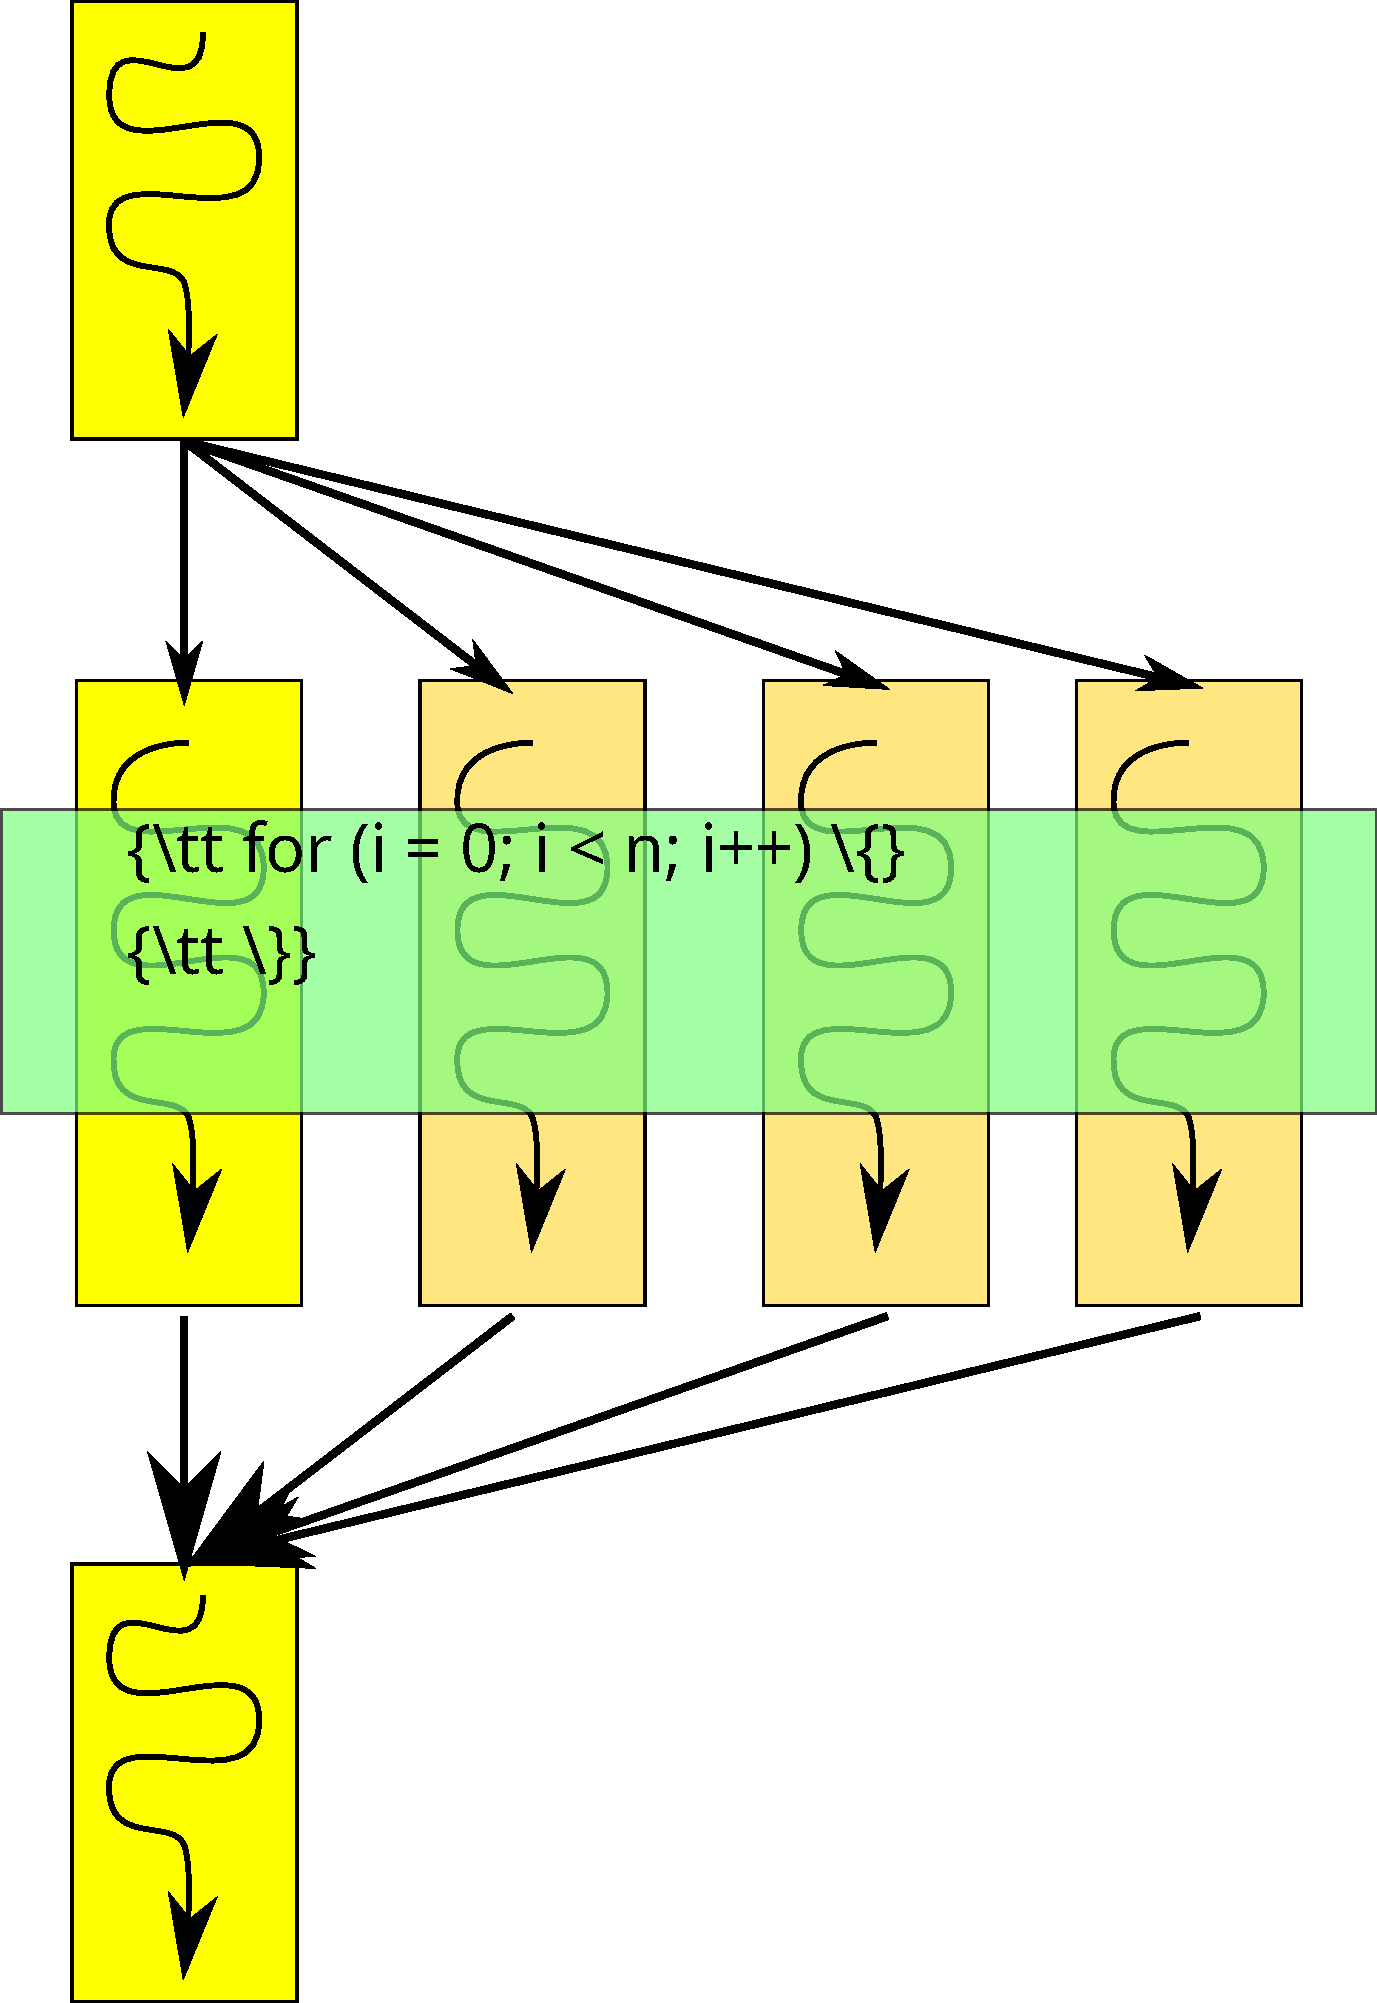
\includegraphics[height=0.7\textheight]{out/pdf/svg/for.pdf}
\def\svgwidth{0.8\textwidth}
{\scriptsize \input{out/tex/svg/for.pdf_tex}}
\end{column}
\end{columns}
\end{frame}

%%%%%%%%%%%%%%%%% 
\begin{frame}[fragile]
\frametitle{{\tt \#pragma omp parallel}}
\begin{columns}
  \begin{column}{0.6\textwidth}
\begin{itemize}
\item basic syntax:
\begin{lstlisting}
  ...
@\ao{\tt \#pragma omp parallel}@
  @$S$@
  ...
\end{lstlisting}
\item basic semantics: 
  \begin{itemize}
  \item create a team of {\tt OMP\_NUM\_THREADS} threads
  \item the current thread becomes the {\em master} of the team
  \item \aka{\em $S$ will be executed by each member of the team}
  \item the master thread waits for all to finish $S$ and continue
  \end{itemize}
\end{itemize}
  \end{column}

  \begin{column}{0.4\textwidth}
%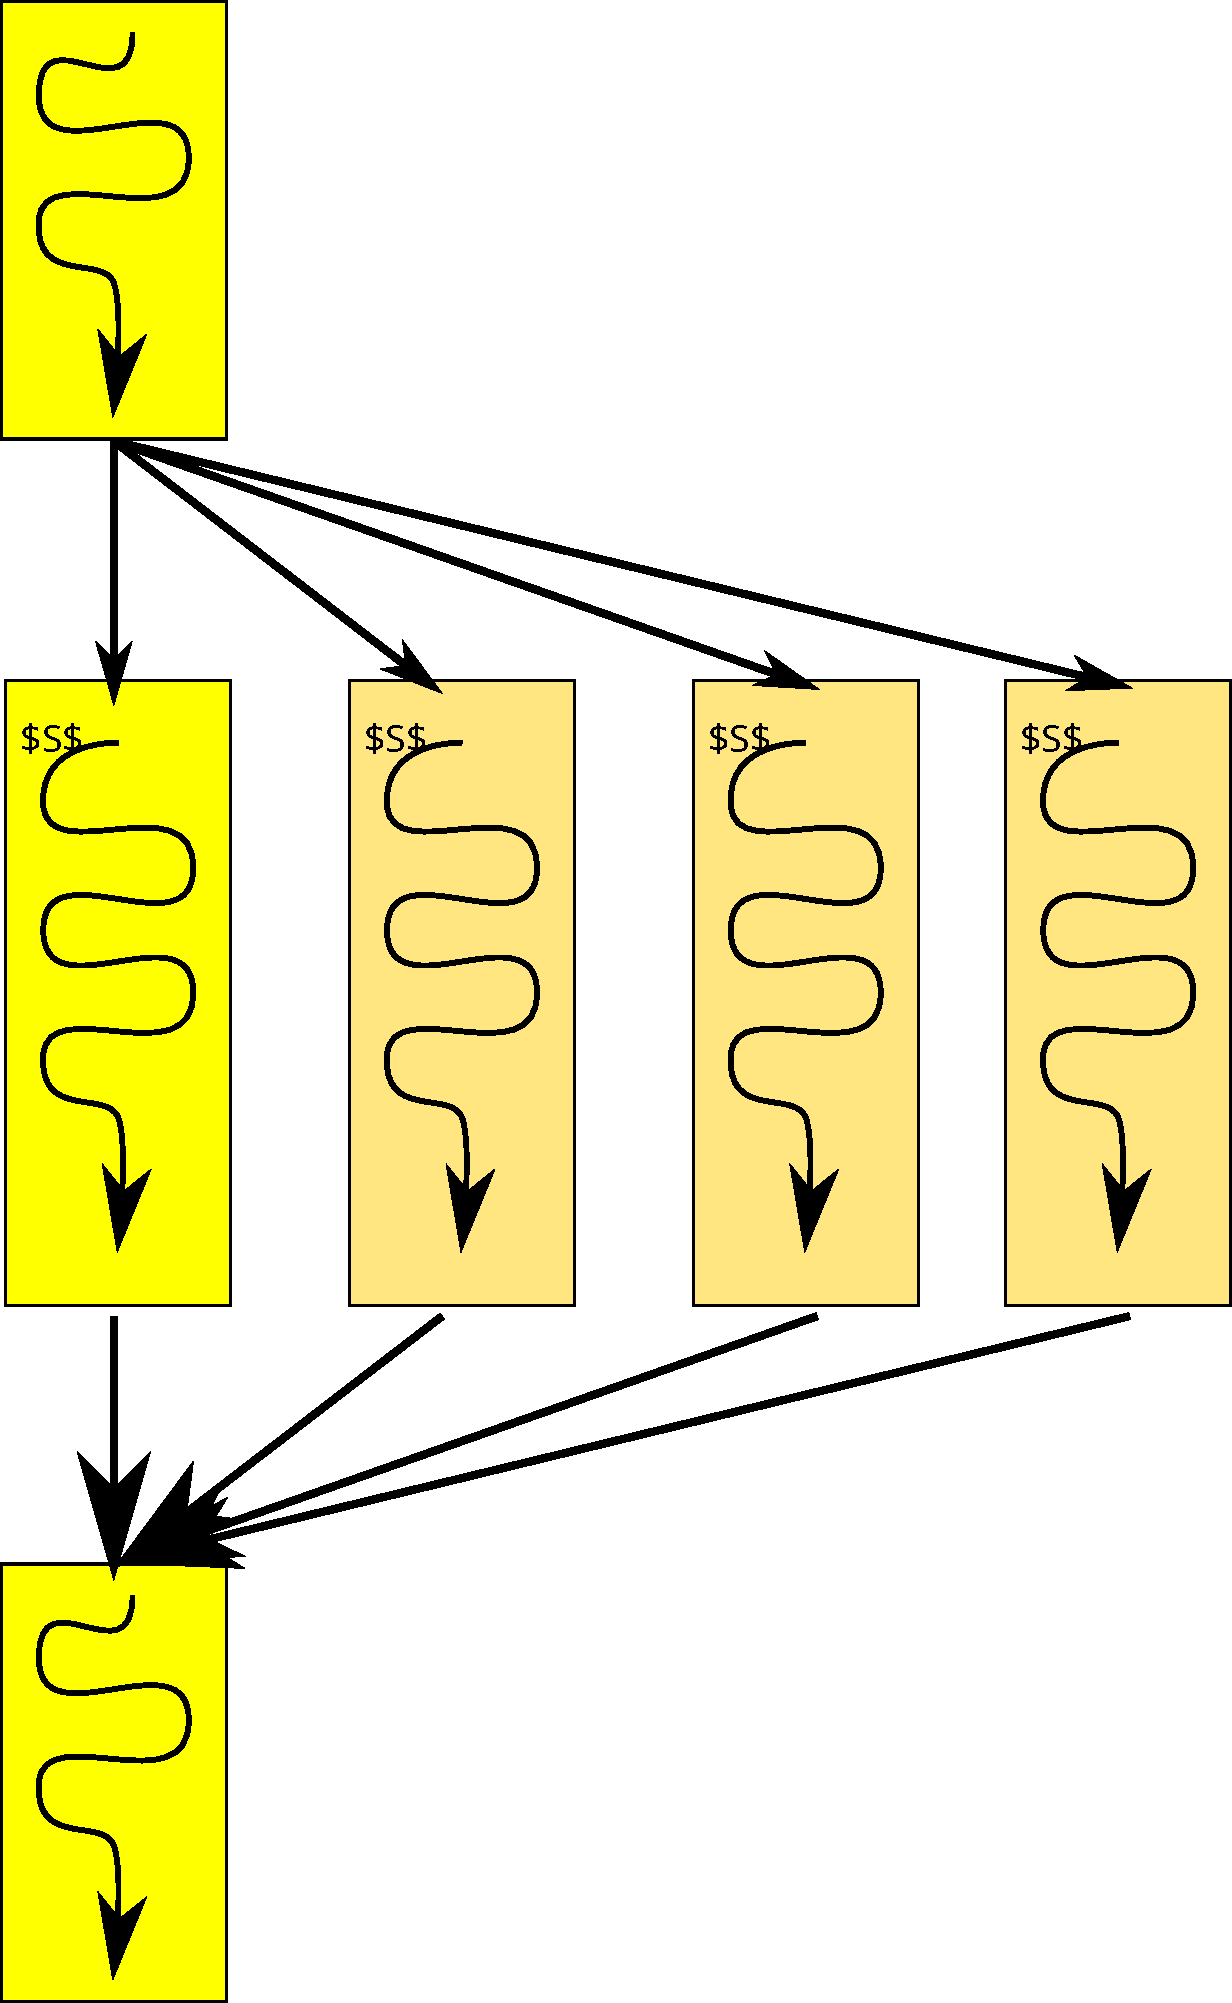
\includegraphics[width=\textwidth]{out/pdf/svg/parallel.pdf}
\def\svgwidth{\textwidth}
{\scriptsize \input{out/tex/svg/parallel.pdf_tex}}
  \end{column}
  
\end{columns}
\end{frame}


%%%%%%%%%%%%%%%%% 
\begin{frame}[fragile]
\frametitle{{\tt parallel} pragma example}

\begin{itemize}
\item []
\begin{lstlisting}
#include <stdio.h>
int main() {
  printf("hello\n");
@\ao{\texttt{\#pragma omp parallel}}@
  printf("world\n");
  printf("bye\n");
  return 0;
}
\end{lstlisting}

\item []
\begin{lstlisting}
$ @\ao{\texttt{OMP\_NUM\_THREADS=1}}@ ./a.out
hello
world
$ @\ao{\texttt{OMP\_NUM\_THREADS=4}}@ ./a.out
hello
world
world
world
world
bye
\end{lstlisting}
\end{itemize}
\end{frame}


\iffalse
%%%%%%%%%%%%%%%%% 
\begin{frame}[fragile]
\frametitle{Remark}

\begin{itemize}
\item []
\begin{lstlisting}
  ...
#pragma omp parallel
  @$S$@
  ...
\end{lstlisting}
\end{itemize}

\begin{itemize}
\item a {\tt parallel} pragma applies to only one statement 
  that immediately follows 
\item you may execute arbitrary number of statements by
  \begin{itemize}
  \item using a compound statement (\{ \ldots \})
\begin{lstlisting}
#pragma omp parallel
{
  ...
  ...
}
\end{lstlisting}
  \item or calling a function in the statement
\begin{lstlisting}
#pragma omp parallel
work();
\end{lstlisting}
  \end{itemize}
\end{itemize}
\end{frame}
\fi

%%%%%%%%%%%%%%%%% 
\begin{frame}[fragile]
\frametitle{Remarks : what does \texttt{parallel} do?}
\begin{itemize}
\item you may assume an OpenMP thread $\approx$ OS-supported 
  thread (e.g., Pthread)

\item that is, if you write this program
\begin{lstlisting}
int main() {
@\ao{\texttt{\#pragma omp parallel}}@
  worker();
}
\end{lstlisting}
and run it as follows,
\begin{lstlisting}
$ @\ao{\texttt{OMP\_NUM\_THREADS=50}}@ ./a.out
\end{lstlisting} %$
you will get 50 OS-level threads, each doing {\tt worker()}
\end{itemize}
\end{frame}

\iffalse
%%%%%%%%%%%%%%%%% 
\begin{frame}[fragile]
\frametitle{Remarks : OpenMP threads vs. TBB tasks}
\begin{itemize}
\item but its function certainly resembles a task in TBB;
  if you think you can use an OpenMP {\tt parallel}
  in place of a TBB task, it's not your fault

\item e.g., 
isn't it a legitimate 
divide-and-conquer merge sort, with OpenMP parallel?
\begin{lstlisting}
void @\ao{\tt ms}@(elem * a, elem * a_end, 
        elem * t, int dest) {
  if (a_end - a == 1) {
    ...
  } else {
    ...
@\ao{\tt \#pragma omp parallel num\_threads(2)}@ // create 2 threads
    {
      if (I am thread #0) ms(a, c,     t,      1 - dest);
      if (I am thread #1) ms(c, a_end, t + nh, 1 - dest);
    }
    ...
  }
}
\end{lstlisting}
\end{itemize}
\end{frame}


%%%%%%%%%%%%%%%%% 
\begin{frame}[fragile]
\frametitle{Remarks : OpenMP threads vs. TBB tasks}

\begin{itemize}
\item the last program just \aka{\em won't work}
\begin{itemize}
\item first of all, OpenMP may not support 
  {\em nested} {\tt parallel} section
  
\item creating an OS-level thread is much more costly than
  creating a task in TBB (or in similar task parallel systems)
  
\item creating so many OS-level threads will yield
  disastrous memory footprint and scheduling order
\end{itemize}

\item just keep in mind; in most programs, 
  you create a fixed number ($\leq$ number of processors) 
  of OpenMP threads and keep them around

\item your mental model when writing OpenMP programs is
\begin{quote}
OpenMP thread $\approx$ processor
\end{quote}

\item very different from the one when 
  writing task-based programs
\end{itemize}
\end{frame}
\fi


%%%%%%%%%%%%%%%%% 
\begin{frame}
\frametitle{How to distribute work among threads?}
\begin{itemize}
\item {\tt \#pragma omp parallel} creates threads, 
  \aka{\em all executing the same statement}
\item it's not a means to parallelize work, {\em per se}, 
  but just a means to create a number of similar threads
  \begin{itemize}
  \item Single Program Multiple Data \ao{(SPMD)} model
  \end{itemize}
  
\item so how to distribute (or partition) work among them?
  \begin{enumerate}
  \item do it yourself
  \item use \ao{\em work sharing} constructs
  \end{enumerate}
\end{itemize}
\end{frame}

%%%%%%%%%%%%%%%%% 
\begin{frame}[fragile]
\frametitle{Do it yourself: functions to get the number/id of threads}

\begin{itemize}
\item \ao{\tt omp\_get\_num\_threads()} 
(\sectionompgetnumthreads) : the number of threads 
  {\em in the current team\/}
\item \ao{\tt omp\_get\_thread\_num()} 
(\sectionompgetthreadnum) : the current thread's id 
  (0, 1, \ldots) in the team
% \item \ao{\tt omp\_get\_max\_threads()} 
% (\sectionompgetmaxthreads) : the number of threads 
%   available if the current thread executes {\tt parallel} pragma

\item they are primitives with which you may
  partition work yourself by whichever ways you
  prefer

\item e.g.,
\begin{lstlisting}
#pragma omp parallel
{
  int t  = omp_get_thread_num();
  int nt = omp_get_num_threads();
  /* divide n iterations evenly amont nt threads */
  for (@\ao{\texttt{i = t * n / nt; i < (t + 1) * n / nt; i++}}@) {
    ...
  }
}
\end{lstlisting}
\end{itemize}
\end{frame}

%=================================
\section{Work sharing constructs}
%=================================

%=================================
\subsection{loops ({\tt for})}
%=================================

%%%%%%%%%%%%%%%%% 
\begin{frame}[fragile]
\frametitle{Work sharing constructs}
\begin{itemize}
\item in theory, \ao{\tt parallel} construct is all you need 
  to do things in parallel
\item but it's too inconvenient
\item OpenMP defines ways to \ao{\em partition} work among threads
  \ao{\em (work sharing constructs)}
  \begin{itemize}
  \item for
  \item task
  \end{itemize}
\end{itemize}
\end{frame}

%%%%%%%%%%%%%%%%% 
\begin{frame}[fragile]
\frametitle{{\tt \#pragma omp for} (work-sharing for)}
\begin{columns}

\begin{column}{0.5\textwidth}
  \begin{itemize}
\item basic syntax (\sectionompfor):
\begin{lstlisting}
@\ao{\tt \#pragma omp for}@
for(i=...; i...; i+=...){
  @$S$@
}
\end{lstlisting}

\item basic semantics:

the threads in the team divde the iterations among them

\item but how? $\Rightarrow$ scheduling
\end{itemize}
\end{column}

\begin{column}{0.5\textwidth}
%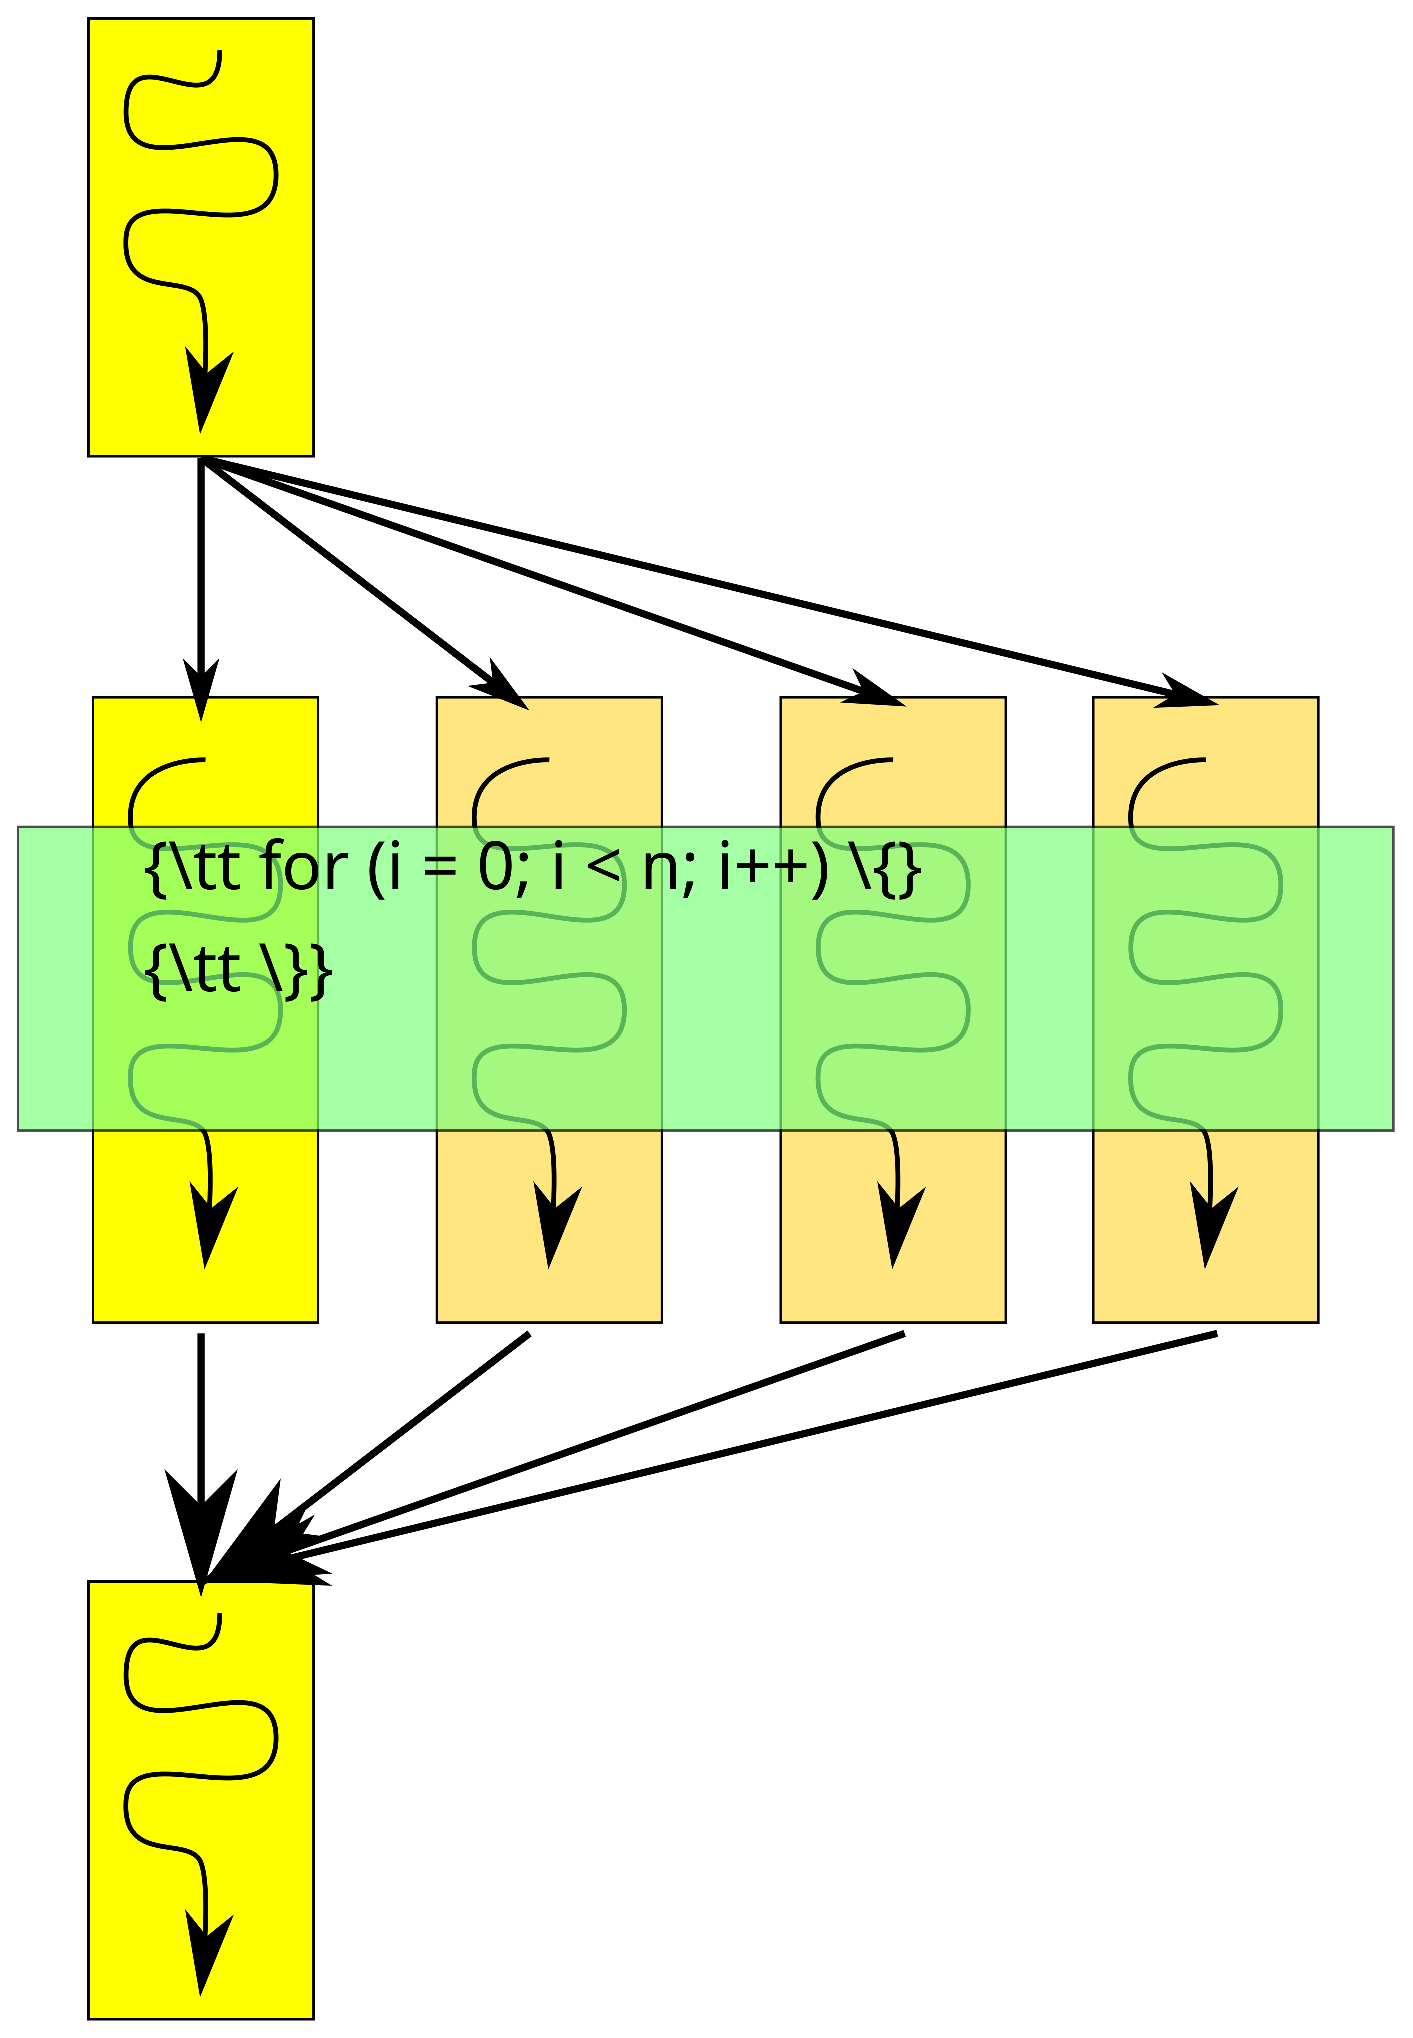
\includegraphics[width=\textwidth]{svg/for.eps}
\def\svgwidth{0.8\textwidth}
{\scriptsize \input{out/tex/svg/for.pdf_tex}}
\end{column}
\end{columns}
\end{frame}

%%%%%%%%%%%%%%%%% 
\begin{frame}[fragile]
\frametitle{{\tt \#pragma omp for} restrictions}
\begin{itemize}
\item iterations are executed in any order may interleave
  \begin{itemize}
  \item the program must not rely on the order in which they are executed
  \end{itemize}
\item strong syntactic restrictions apply (\sectionompforform); basically,
\ao{\em the iteration space must be easily 
  identifiable at the beginning\/} of the loop
\begin{itemize}
\item roughly, it must be of the form:
\begin{lstlisting}
#pragma omp for
for(i = @{\em init}@; i < @{\em limit}@; i += @{\em incr}@) 
  @$S$@
\end{lstlisting}
except {\tt <} and {\tt +=} may be other similar operators
\item {\em init}, {\em limit}, and {\em incr} must be loop invariant
\end{itemize}
\end{itemize}
\end{frame}

%%%%%%%%%%%%%%%%% 
\begin{frame}[fragile]
\frametitle{Parallel SpMV for CSR using {\tt \#pragma omp for}}
\begin{itemize}
\item it only takes to work-share the outer for loop
\begin{lstlisting}
// assume inside @\ao{\tt \#pragma omp parallel}@
   ...
@\ao{\tt \#pragma omp for}@
for (i = 0; i < A.n_rows; i++) {
  for (k = A.row_start[i]; k < A.row_start[i+1]; k++) {
    j,Aij = A.elems[k];
    y[i] += Aij * x[j];
  }
}
\end{lstlisting}

\item note: the inner loop ($k$) is executed sequentially
\end{itemize}
\end{frame}


%%%%%%%%%%%%%%%%% 
\begin{frame}[fragile]
  \frametitle{Parallel SpMV COO using {\tt \#pragma omp for}?}
  \begin{itemize}
  \item the following code does {\it not} work (why?)
\begin{lstlisting}
// assume inside @\ao{\tt \#pragma omp parallel}@
   ...
@\aka{\tt \#pragma omp for}@
for (k = 0; k < A.nnz; k++) {
  i,j,Aij = A.elems[k];
  @\aka{\tt y[i]}@ += Aij * x[j];
}
\end{lstlisting}

\item a possible remedy will be described later
  \end{itemize}
\end{frame}

%=================================
\subsection{scheduling}
%=================================

%%%%%%%%%%%%%%%%% 
\begin{frame}[fragile]
\frametitle{Scheduling (\sectionompfor)}
\begin{itemize}
\item \ao{\tt schedule} clause in work-sharing for loop determines
how iterations are divided among threads
\item There are three alternatives 
  (\ao{\tt static, dynamic,} and \ao{\tt guided})
\end{itemize}
\end{frame}


%%%%%%%%%%%%%%%%% 
\begin{frame}
\frametitle{static, dynamic, and guided}
\begin{columns}[t]
  \begin{column}{0.53\textwidth}
\begin{itemize}
\item {\tt schedule(\ao{static{\rm [,{\em chunk}]}})}: 
  predictable round-robin
\item {\tt schedule(\ao{dynamic{\rm [,{\em chunk}]}})}:
  each thread repeats fetching {\em chunk} iterations
\item {\tt schedule(\ao{guided{\rm [,{\em chunk}]}})}:
  threads grab many iterations in early stages;
  gradually reduce iterations to fetch at a time

\item \ao{\em chunk} specifies the minimum granularity
  (iteration counts)
\end{itemize}
  \end{column}

  \begin{column}{0.47\textwidth}
%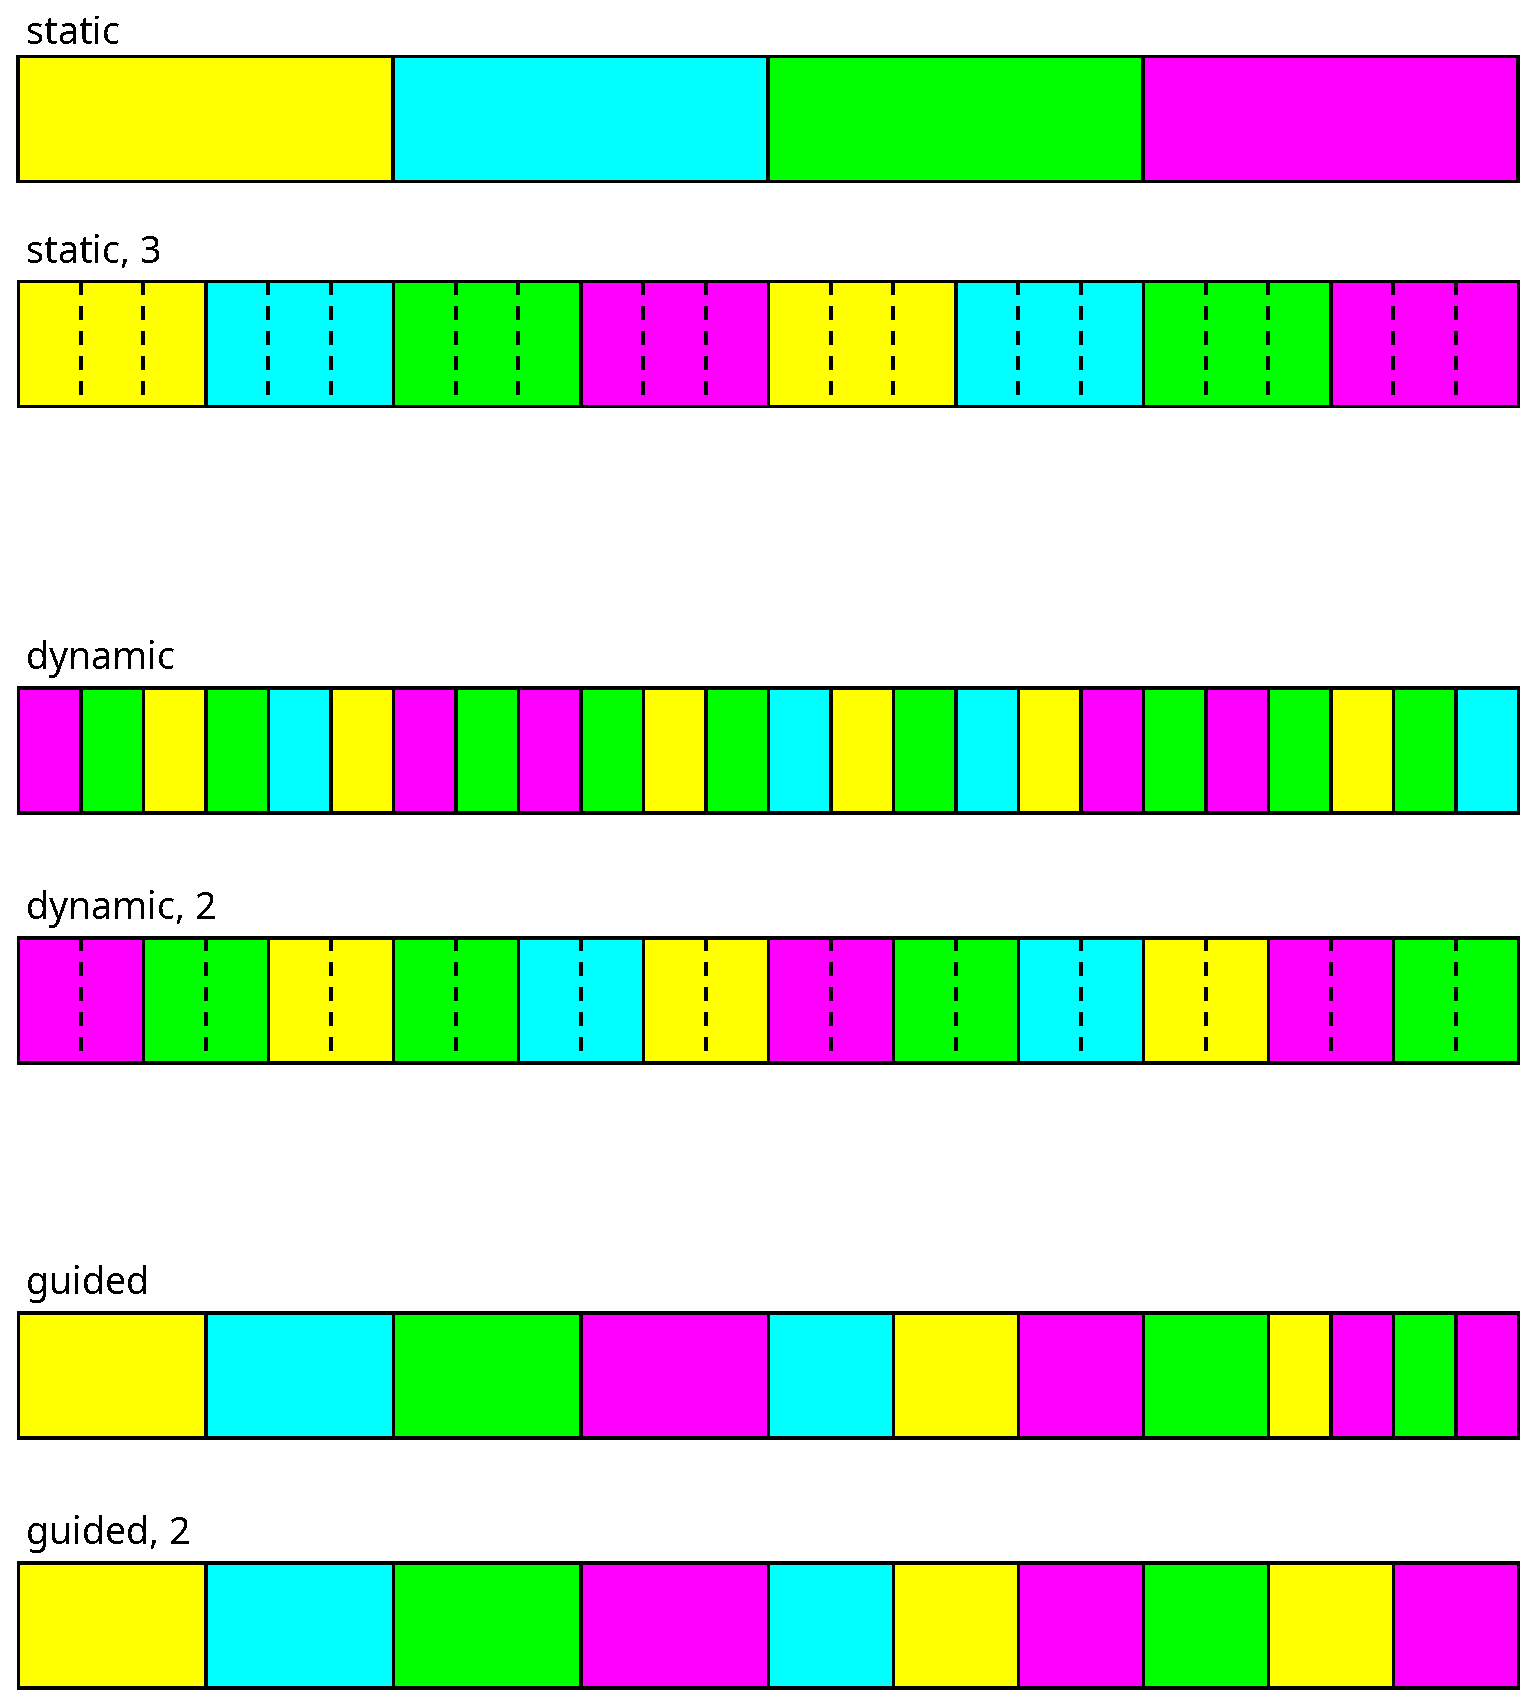
\includegraphics[width=\textwidth]{svg/scheduler.eps}
\def\svgwidth{\textwidth}
{\scriptsize \input{out/tex/svg/scheduler.pdf_tex}}
  \end{column}
\end{columns}
\end{frame}

%%%%%%%%%%%%%%%%% 
\begin{frame}[fragile]
\frametitle{Other scheduling options and notes}
\begin{itemize}
\item {\tt schedule(\ao{runtime})} determines the schedule by
  {\tt OMP\_SCHEDULE} environment variable. e.g.,
\begin{lstlisting}
$ OMP_SCHEDULE=dynamic,2 ./a.out
\end{lstlisting} %$

\item {\tt schedule(\ao{auto})} or \ao{no {\tt schedule} clause} choose
  an implementation dependent default

% \item \ao{\em caution: is this a gcc bug?}
% \begin{lstlisting}
% $ OMP_SCHEDULE=static ./a.out
% \end{lstlisting} %$ 
% appears to mean {\tt schedule(\ao{static,1})}, not {\tt schedule(static)}

\end{itemize}
\end{frame}

%%%%%%%%%%%%%%%%% 
\begin{frame}[fragile]
\frametitle{Parallelizing loop nests by \ao{\tt collapse}}
\begin{itemize}
\item \ao{\tt collapse($l$)} can be used to partition nested loops. e.g.,
\begin{lstlisting}
#pragma omp for @\ao{collapse(2)}@
for (i = 0; i < n; i++)
  for (j = 0; j < n; j++)
    @$S$@
\end{lstlisting}
will partition $n^2$ iterations of the doubly-nested loop
\item {\tt schedule} clause applies to nested loops as if 
  the nested loop is an equivalent flat loop
\item restriction: the loop must be \ao{\em ``perfectly nested''}
  (the iteration space must be a rectangular and no intervening
  statement between different levels of the nest)
\end{itemize}
\end{frame}


%%%%%%%%%%%%%%%%% 
\begin{frame}[fragile]
\frametitle{Visualizing schedulers}
\begin{itemize}
\item seeing is believing. let's visualize how loops are distributed among threads
\item write a simple doubly nested loop and run it under various scheduling options
\begin{lstlisting}
#pragma omp for collapse(2) schedule(runtime)
for (i = 0; i < 1000; i++)
  for (j = 0; j < 1000; j++)
    unit_work(i, j);
\end{lstlisting}
\end{itemize}


\begin{columns}
\begin{column}{0.6\textwidth}
\begin{itemize}
\item load per point is systematically skewed:
  \begin{itemize}
  \item $\approx 0$ in the lower triangle
  \item randomly drawn from $[100,10000]$ (clocks) in the upper triangle
  \end{itemize}
\end{itemize}  
\end{column}

\begin{column}{0.4\textwidth}
\begin{center}
%\includegraphics[width=0.3\textwidth]{out/pdf/img/loadbalance_vis.pdf}
\def\svgwidth{\textwidth}
{\scriptsize \input{out/tex/svg/scheduler_vis_dynamic.pdf_tex}}
\end{center}
\end{column}
\end{columns}
\end{frame}


%%%%%%%%%%%%%%%%% 
\begin{frame}
\frametitle{Visualizing schedulers}
\begin{columns}
\begin{column}{0.5\textwidth}
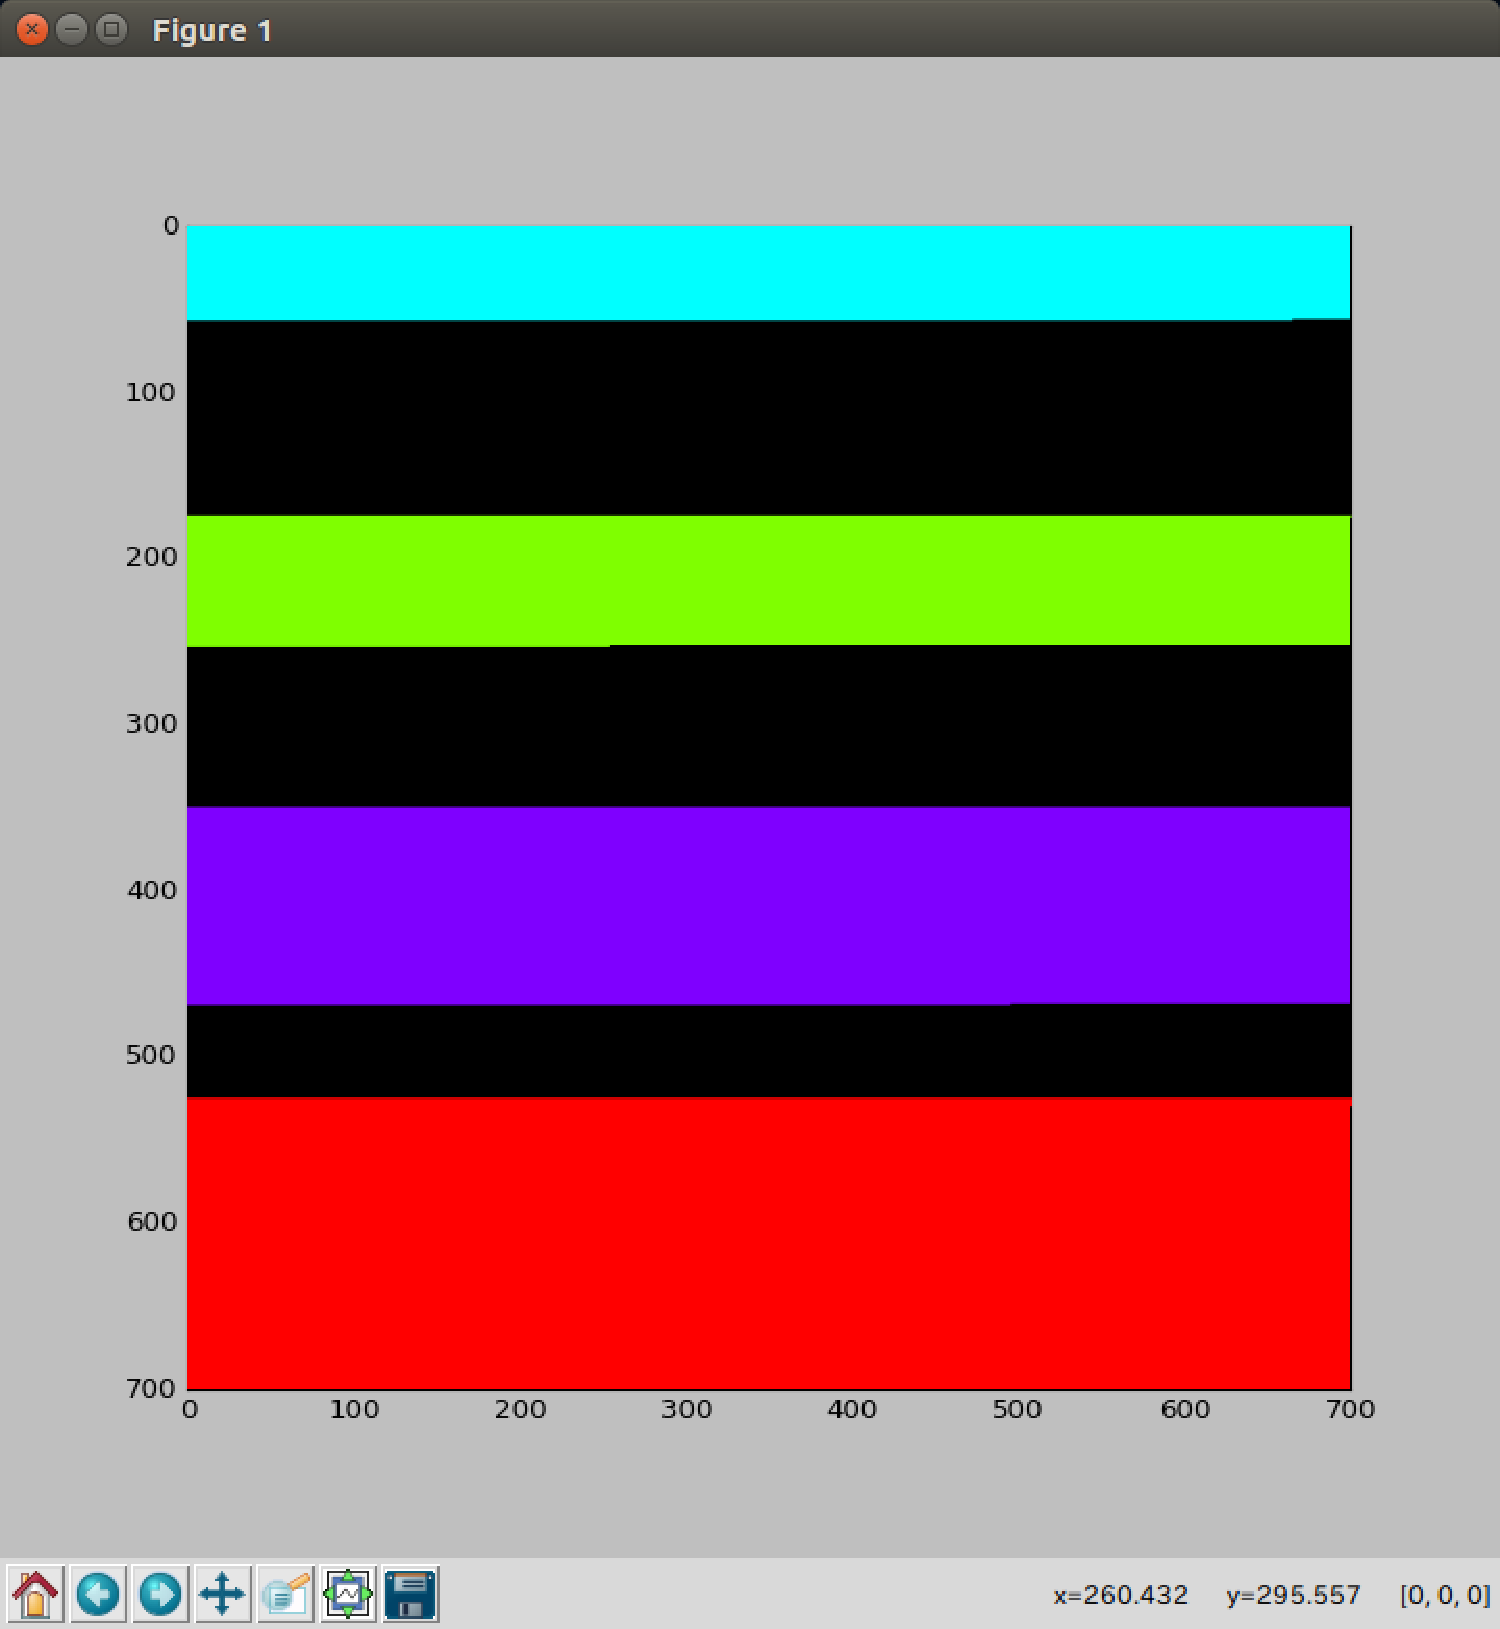
\includegraphics[width=\textwidth]{out/pdf/img/load_balance_static.pdf}
\vskip-2mm
{\footnotesize static}
\end{column}

\begin{column}{0.5\textwidth}
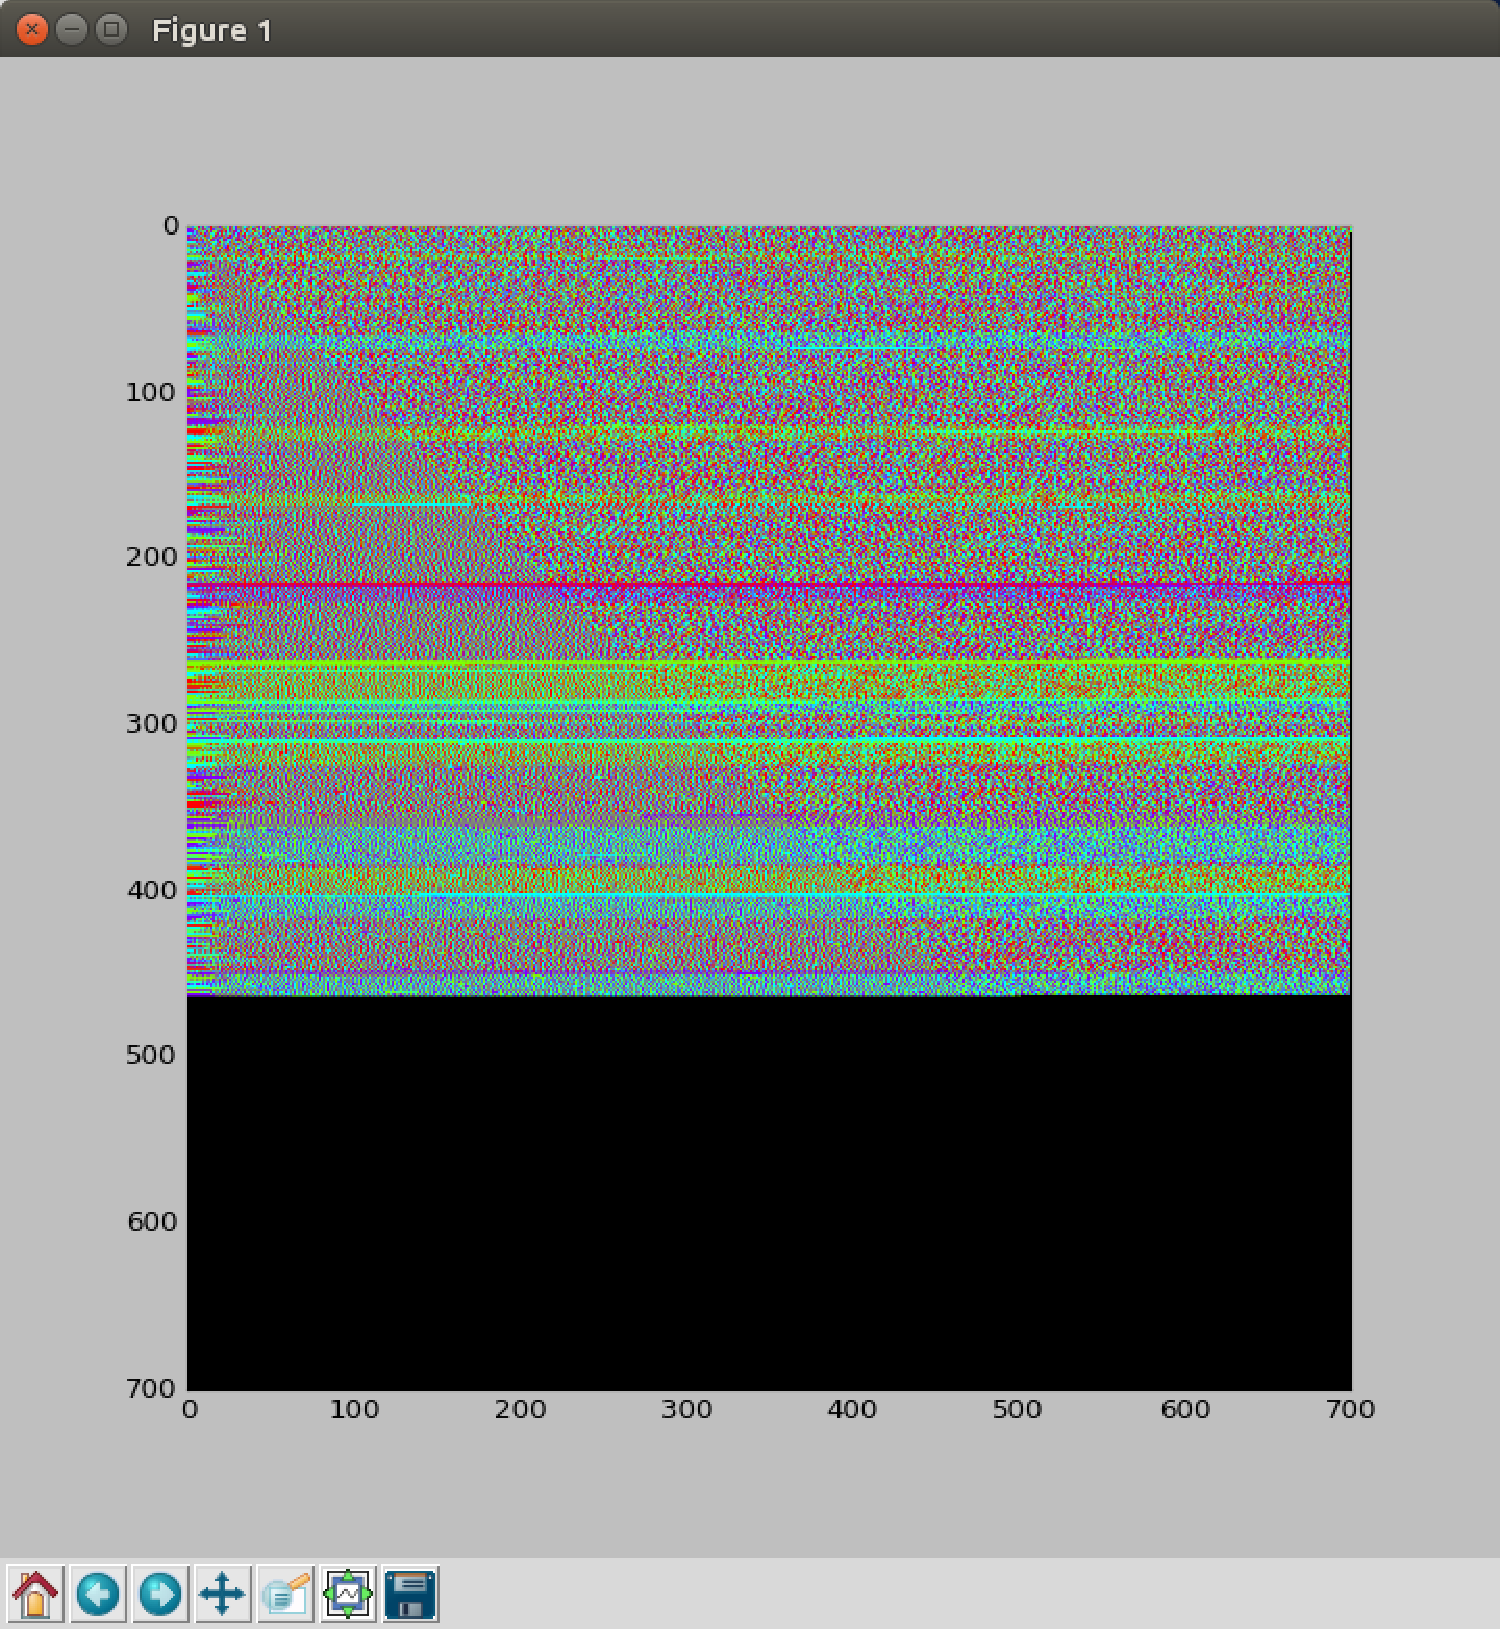
\includegraphics[width=\textwidth]{out/pdf/img/load_balance_dynamic.pdf}
\vskip-2mm
{\footnotesize dynamic}
\end{column}
\end{columns}
\end{frame}

%%%%%%%%%%%%%%%%% 
\begin{frame}[fragile]
  \frametitle{Scheduling for SpMV on CSR}
  \begin{itemize}
  \item []
\begin{lstlisting}
// assume inside @\ao{\tt \#pragma omp parallel}@
   ...
@\ao{\tt \#pragma omp for schedule(\aka{???})}@
for (i = 0; i < A.n_rows; i++) {
  for (k = A.row_start[i]; k < A.row_start[i+1]; k++) {
    j,Aij = A.elems[k];
    y[i] += Aij * x[j];
  }
}
\end{lstlisting}
\item \ao{static?} depending on the number of elements in rows,
    load imbalance may be significant
 \item \ao{dynamic/guided?} load balancing will be better,
    but extremely dense rows may still be an issue
\item the more robust strategy is to partition non-zeros, not rows
  \end{itemize}
\end{frame}

% =================================
\subsection{task parallelism ({\tt task} and {\tt taskwait})}
%=================================

%%%%%%%%%%%%%%%%% 
\begin{frame}[fragile]
\frametitle{Task parallelism in OpenMP}
\begin{itemize}
\item OpenMP's initial focus was simple parallel loops
\item since 3.0, it supports task parallelism
\item but why it's necessary?
\item aren't \texttt{parallel} and \texttt{for} all we need?
\end{itemize}
\end{frame}

%%%%%%%%%%%%%%%%% 
\begin{frame}[fragile]
\frametitle{Limitation of \texttt{parallel for}}
\begin{columns}
\begin{column}{0.5\textwidth}
\begin{itemize}
\item what if you have a parallel loop inside another
\begin{lstlisting}
@\ao{\texttt for}@ ( ... ) {
  ...
  @\ao{\texttt for}@ ( ...) ...
}
\end{lstlisting}

\item perhaps in a function?
\begin{lstlisting}
main() {
  @\ao{\texttt for}@ ( ... ) {
    ...
    g();
  }
}
g() { 
  @\ao{\texttt for}@ (...) ...
}
\end{lstlisting}
\end{itemize}
\end{column}
  
\begin{column}{0.5\textwidth}
\begin{itemize}
\item what about parallel recursions?
\begin{lstlisting}
@\ao{\texttt qs}@() {
  if (...) { ... }
  else {
    @\ao{\texttt qs}@();
    @\ao{\texttt qs}@();
  }
}      
\end{lstlisting}
\end{itemize}

\begin{center}
%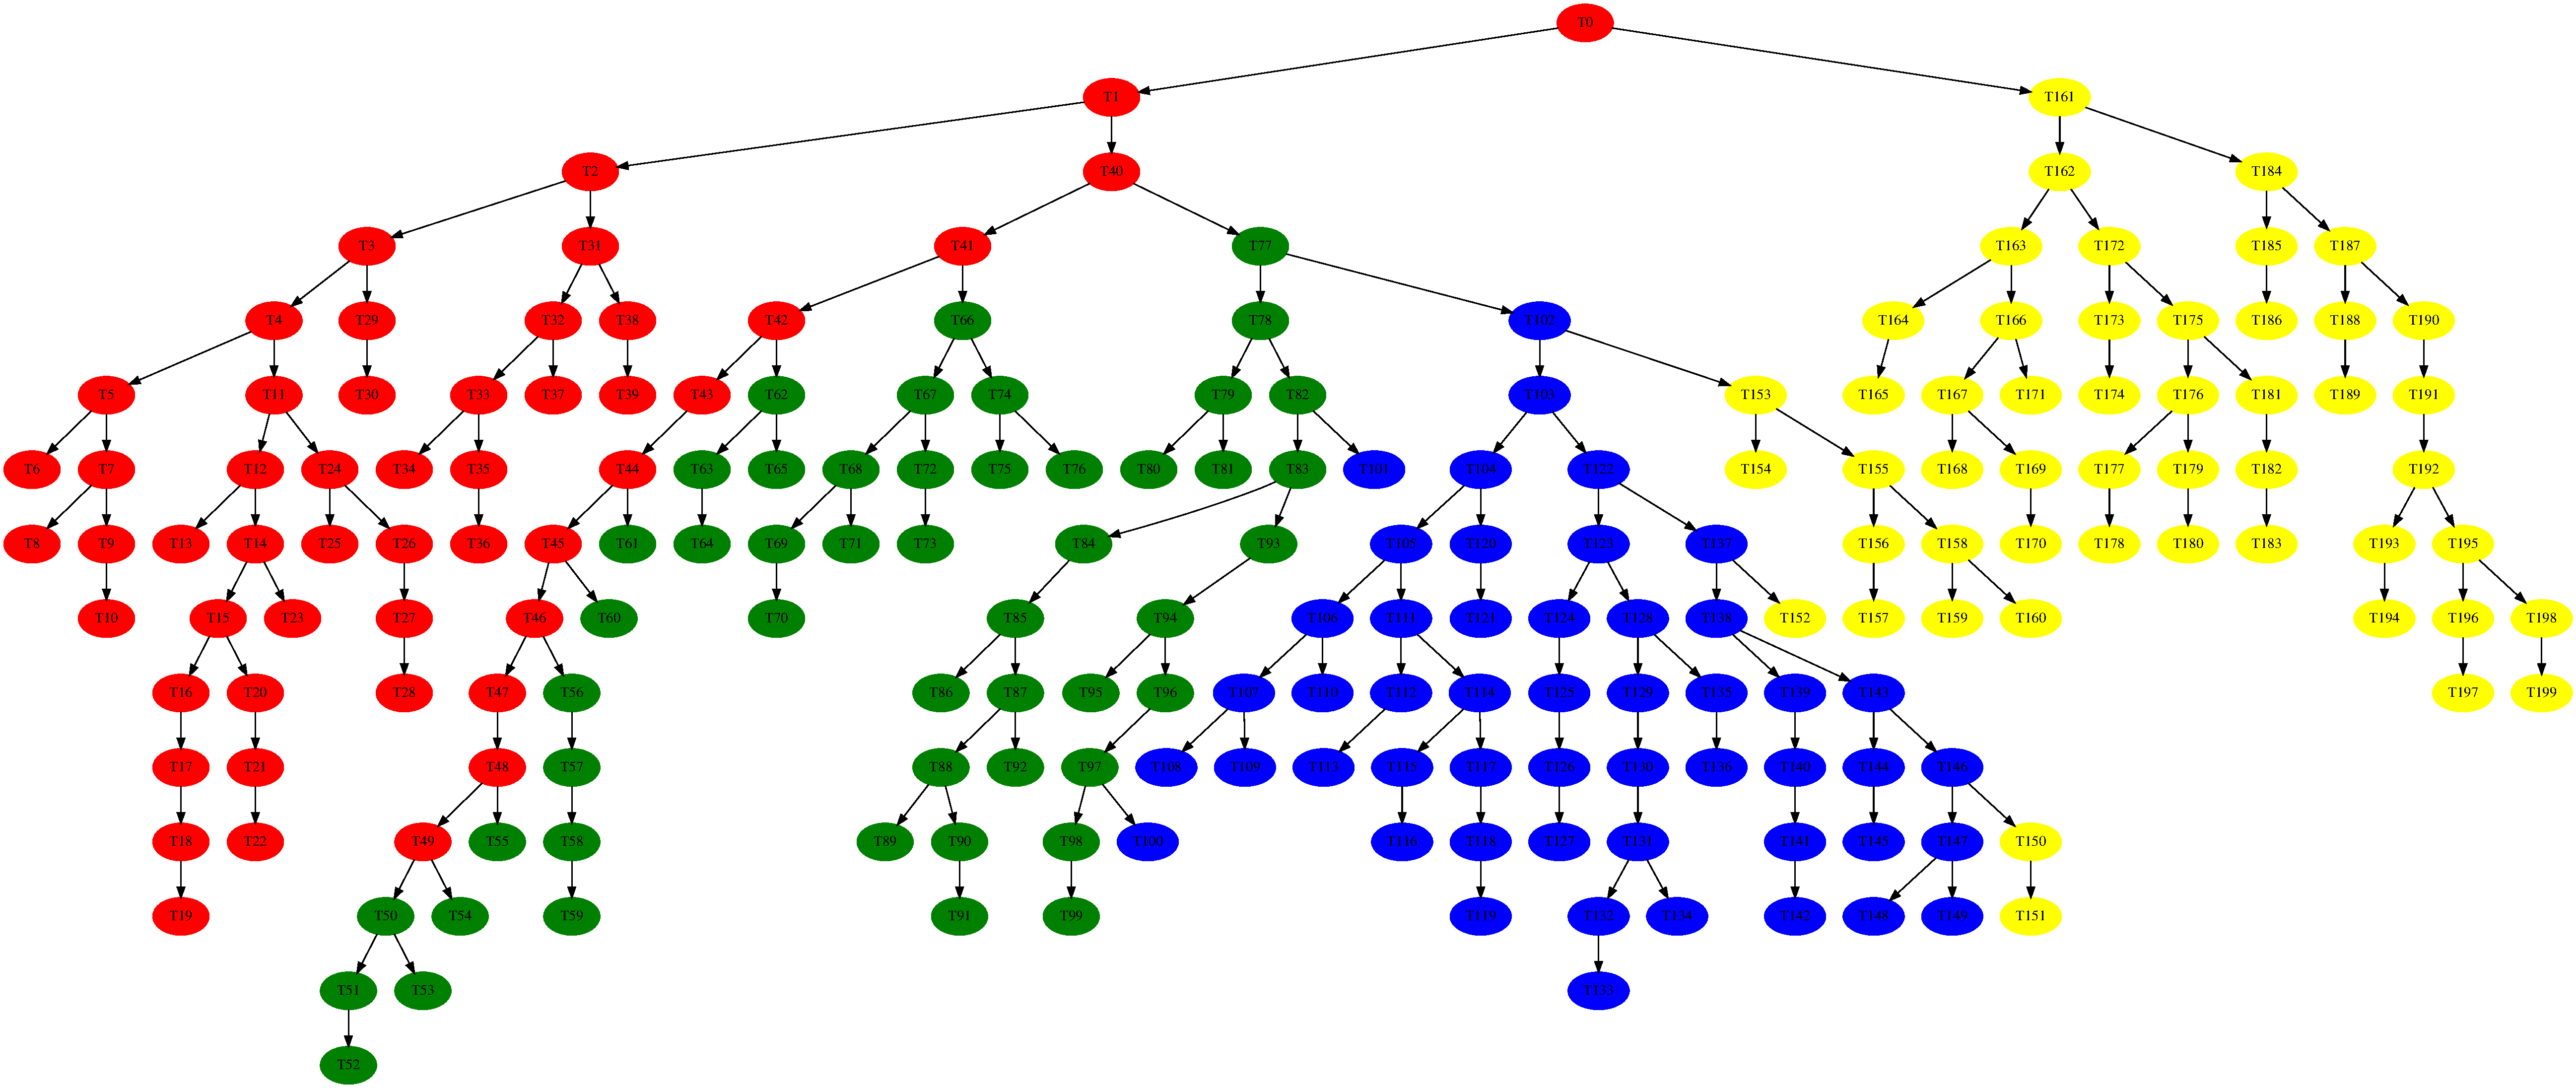
\includegraphics[width=0.8\textwidth]{out/pdf/svg/randtree.pdf}
\end{center}

\end{column}
\end{columns}
\end{frame}


%%%%%%%%%%%%%%%%% 
\begin{frame}
\frametitle{\texttt{parallel for} can't handle nested parallelism}
\begin{columns}
  \begin{column}{0.6\textwidth}
\begin{itemize}
\item<1-> OpenMP generally ignores nested
  \texttt{parallel} pragma when enough
  threads have been created by the outer
  \texttt{parallel} pragma, for good reasons

\item<2-> the fundamental limitation is its
  simplistic work-sharing mechanism

\item<3-> \ao{\it tasks} address these issues, by allowing tasks
  to be created at arbitrary points of execution
  (and a mechanism to distribute them across cores)
\end{itemize}
  \end{column}

\begin{column}{0.4\textwidth}
%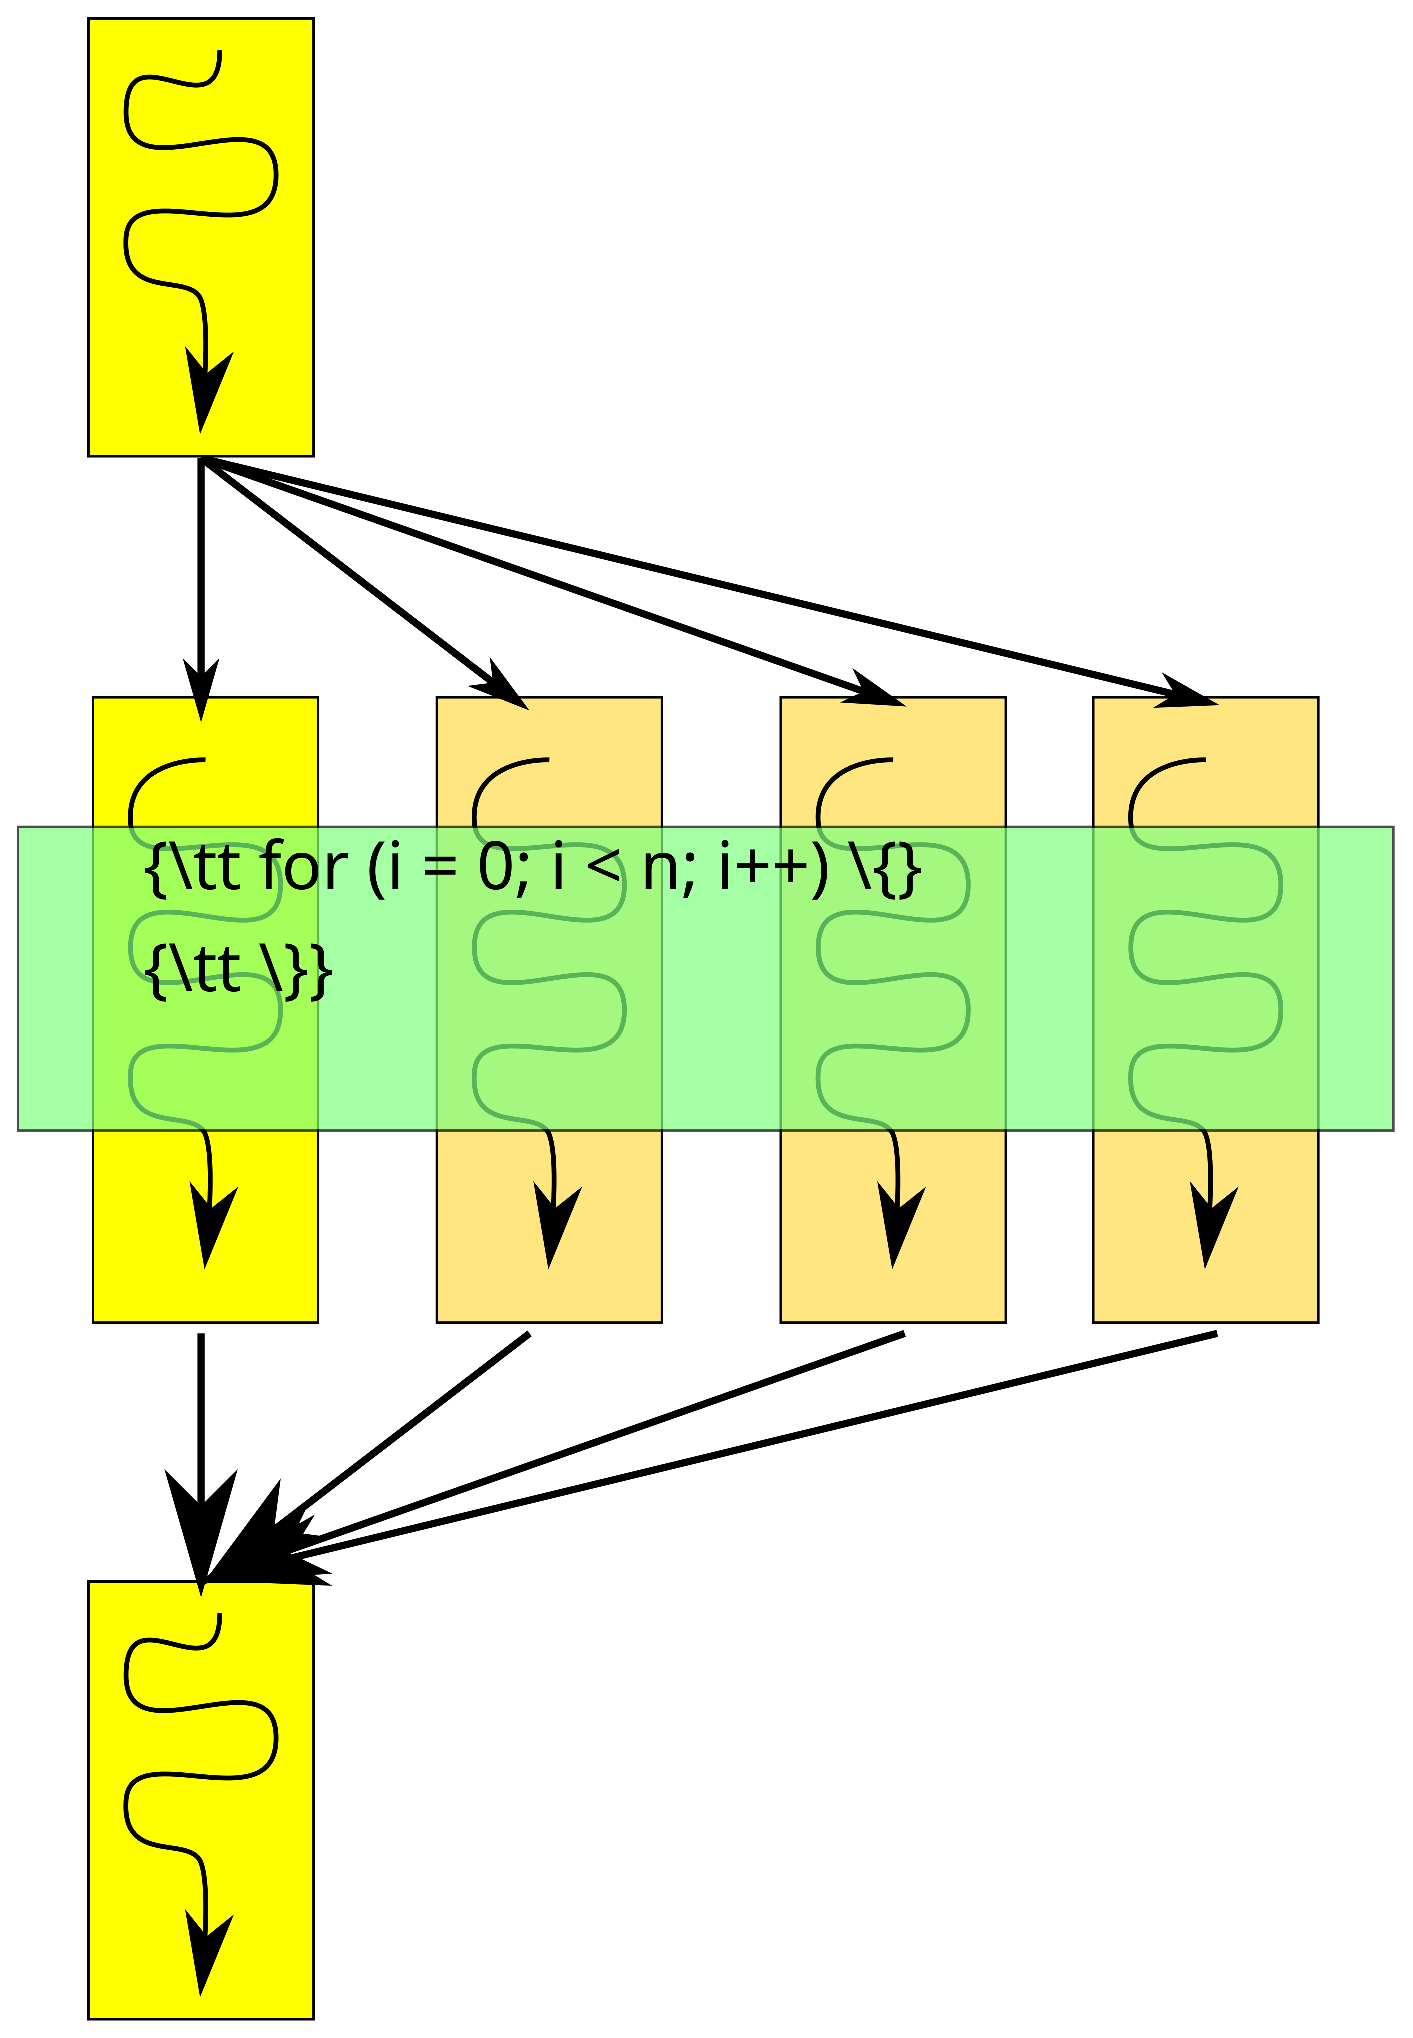
\includegraphics[width=\textwidth]{svg/for.eps}
\def\svgwidth{\textwidth}
{\scriptsize \input{out/tex/svg/for.pdf_tex}}
\end{column}
\end{columns}
\end{frame}



%%%%%%%%%%%%%%%%% 
\begin{frame}[fragile]
\frametitle{Task parallelism in OpenMP}
\begin{itemize}
\item syntax:
  \begin{itemize}
  \item {\tt task} creates a task executing $S$ (\sectionomptask)
\begin{lstlisting}
@\ao{\tt \#pragma omp task}@
  @$S$@
\end{lstlisting}
\item {\tt taskwait} waits for child tasks to finish (\sectionomptaskwait)
\begin{lstlisting}
@\ao{\tt \#pragma omp taskwait}@
\end{lstlisting}
  \end{itemize}
\end{itemize}
\end{frame}

%%%%%%%%%%%%%%%%% 
\begin{frame}[fragile]
\frametitle{OpenMP task parallelism template}
\begin{columns}[t]
\begin{column}{0.48\textwidth}
\begin{itemize}
\item don't forget to create a \ao{\texttt{parallel}} region 
%  {\tiny (otherwise everything will be done by a single thread)}
\item don't also forget to enter a \ao{\texttt{master}} region, which says
  only the master executes the following statement
  and others ``stand-by'' 
% {\tiny (to execute creasted tasks;
%    otherwise \ao{\em every} thread will duplicate the same tasks)}
\begin{lstlisting}
int main() {
@\ao{\tt \#pragma omp parallel}@
@\ao{\tt \#pragma omp master}@
// or @{\tt \#pragma omp single}@
  ms(a, a + n, t, 0);
}
\end{lstlisting}
\end{itemize}
\end{column}

\begin{column}{0.52\textwidth}
\begin{itemize}
\item and create tasks in the master region
\begin{lstlisting}
void ms(a, a_end, t, dest) {
  if (n == 1) {
    ...
  } else {
    ...
#pragma omp task
    ms(a, c,     t,      1 - dest);
#pragma omp task
    ms(c, a_end, t + nh, 1 - dest);
#pragma omp taskwait
    ...
}
\end{lstlisting}
\end{itemize}
\end{column}
\end{columns}
\end{frame}

%%%%%%%%%%%%%%%%% 
\begin{frame}
  \frametitle{What are tasks good for?}
  \begin{itemize}
  \item the strength of tasks as opposed to for loop is its flexibility
    \begin{itemize}
    \item create tasks at any point during the computation
    \item they get distributed to cores
    \end{itemize}
  \item especially good for ``nested parallelism'' and ``parallel recursions
    (divide and conquer)''
  \end{itemize}

  \begin{center}
    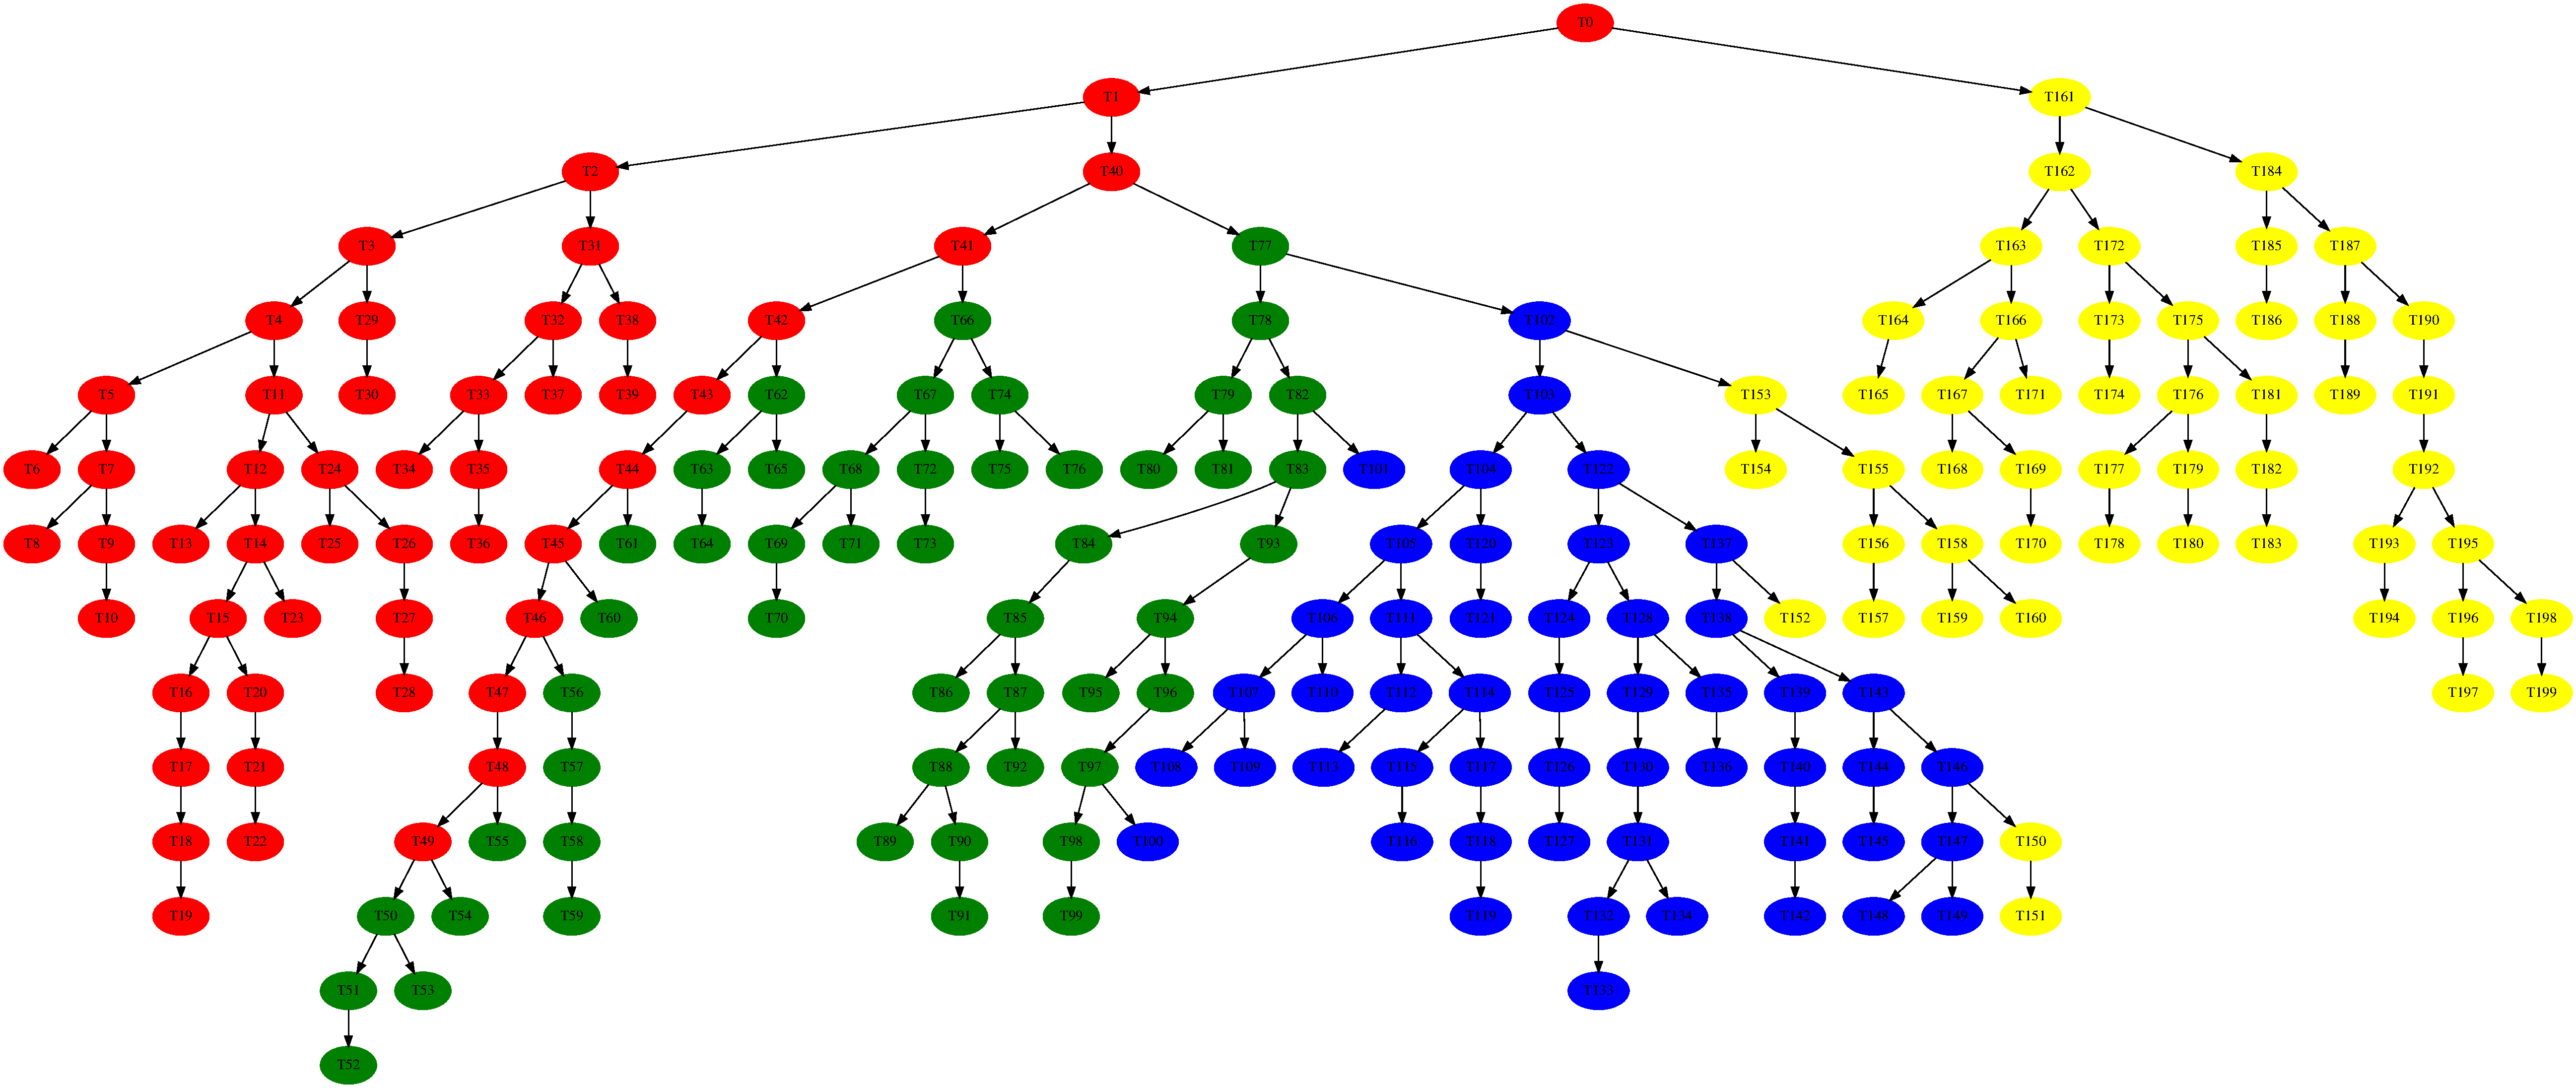
\includegraphics[width=0.6\textwidth]{out/pdf/svg/randtree.pdf}
%  \def\svgwidth{0.6\textwidth}
%  {\scriptsize \input{out/tex/svg/randtree.pdf_tex}}
  \end{center}

  \begin{itemize}
  \item even for loops, you may consider reformulating
    them into divide-and-conquer as an alternative dynamic
    load-balancing strategy
  \end{itemize}
\end{frame}

%%%%%%%%%%%%%%%%% 
\begin{frame}[fragile]
\frametitle{Visualizing task parallel schedulers}
\begin{columns}
\begin{column}{0.7\textwidth}
\begin{itemize}
\item the workload is exactly the same as before
\begin{lstlisting}
#pragma omp for collapse(2) schedule(runtime)
for (i = 0; i < 1000; i++)
  for (j = 0; j < 1000; j++)
    unit_work(i, j);
\end{lstlisting}
\item but we rewrite it into recursions
\begin{lstlisting}
void work_rec(rectangle b) {
  if (small(b)) {
    ...
  } else {
    rectangle c[2][2];
    split(b, c); // split b into 2x2 sub-rectangles
    for (i = 0; i < 2; i++) {
      for (i = 0; i < 2; i++) {
#pragma omp task 
        work_rec(b[i][j]);
      }
    }
#pragma omp taskwait
  }
}
\end{lstlisting}
\end{itemize}
\end{column}

\begin{column}{0.3\textwidth}
\begin{center}
\def\svgwidth{\textwidth}
{\scriptsize \input{out/tex/svg/scheduler_vis.pdf_tex}}
\end{center}
\end{column}
\end{columns}
\end{frame}

%%%%%%%%%%%%%%%%% 
\begin{frame}
\frametitle{Visualizing schedulers}
\begin{center}
\begin{columns}
  \begin{column}{0.3\textwidth}
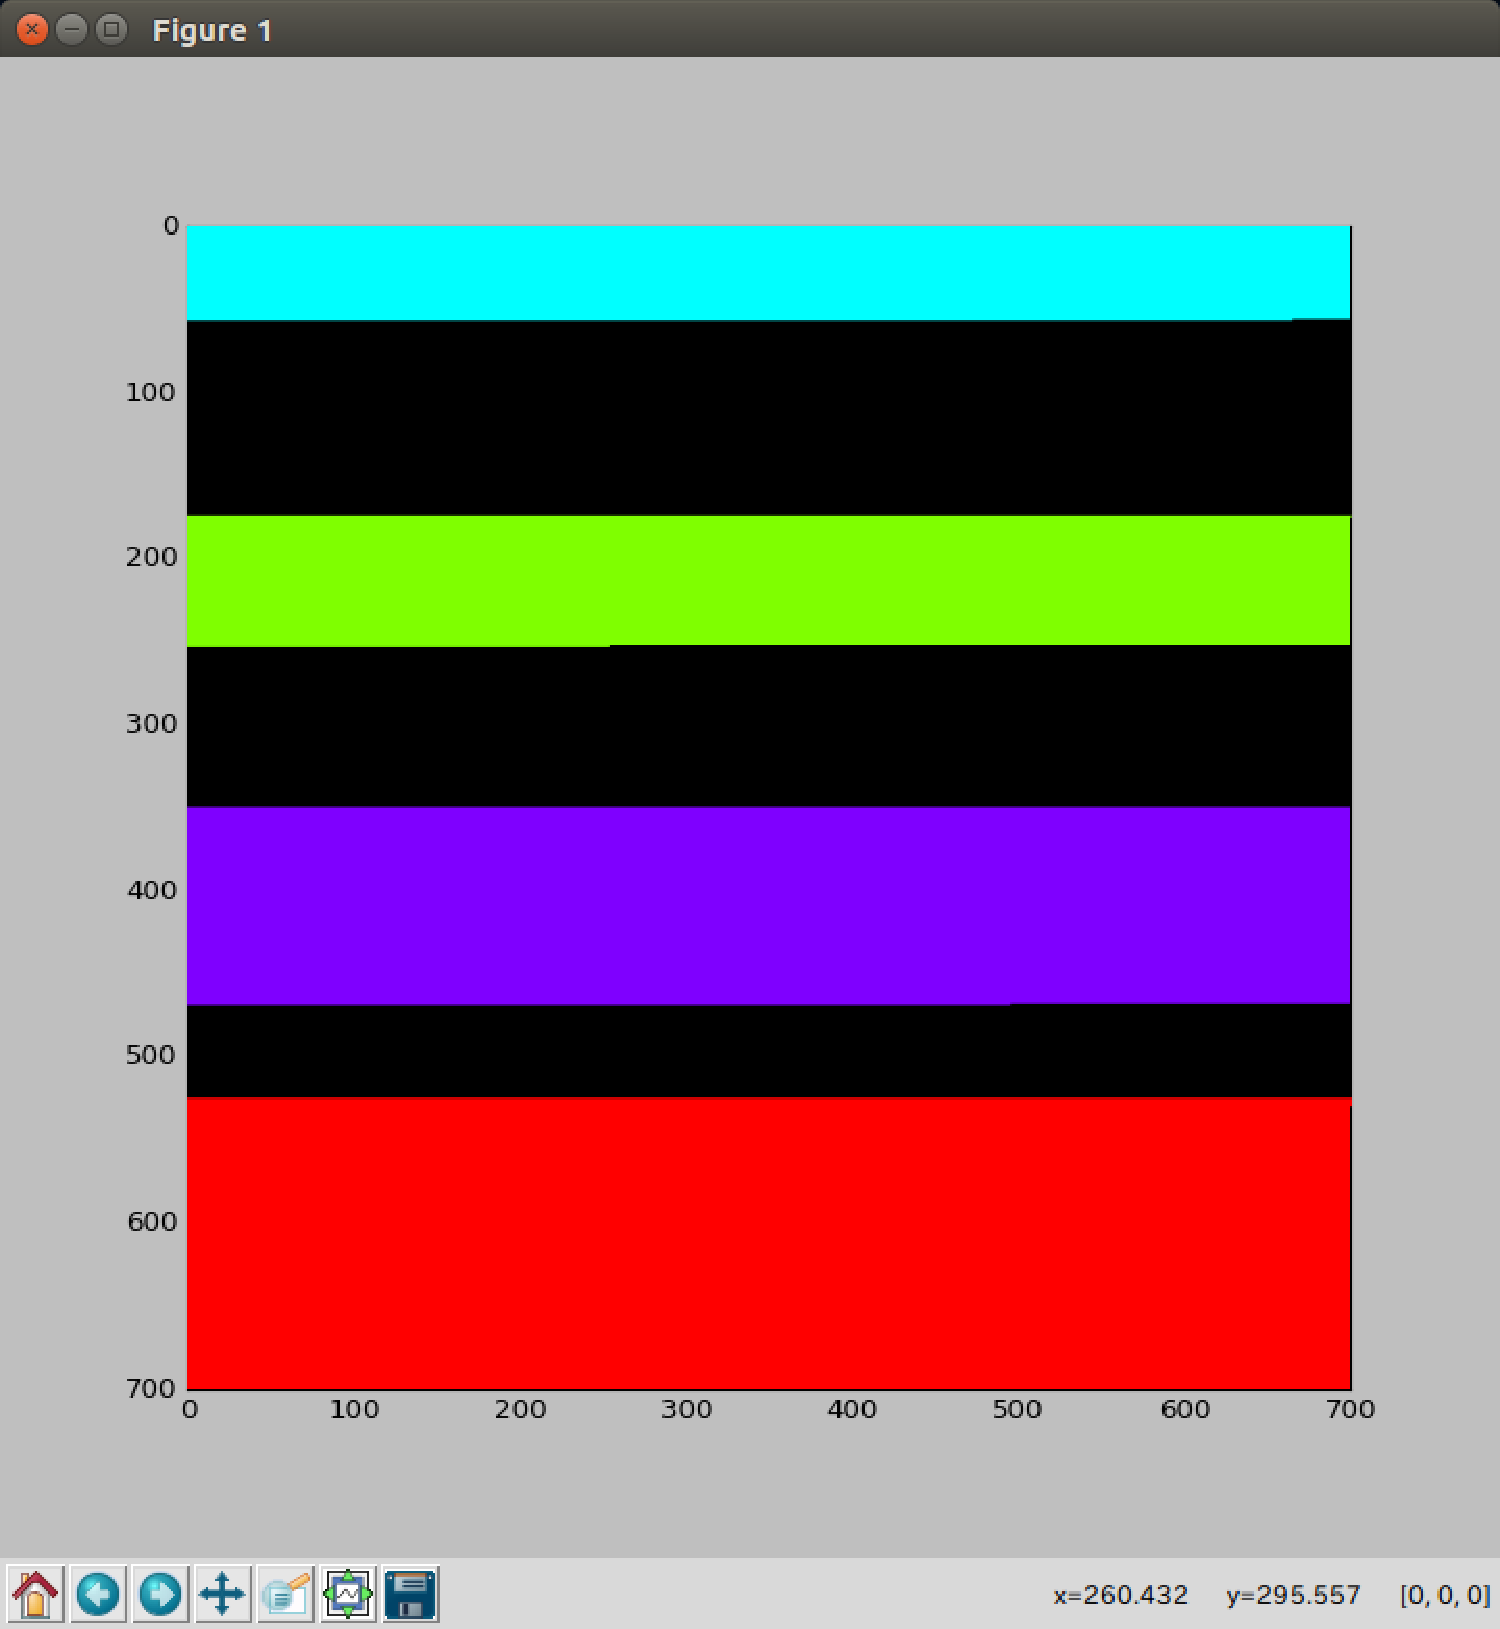
\includegraphics[width=0.8\textwidth]{out/pdf/img/load_balance_static.pdf}
\vskip-2mm
{\footnotesize static}
    
\vskip3mm

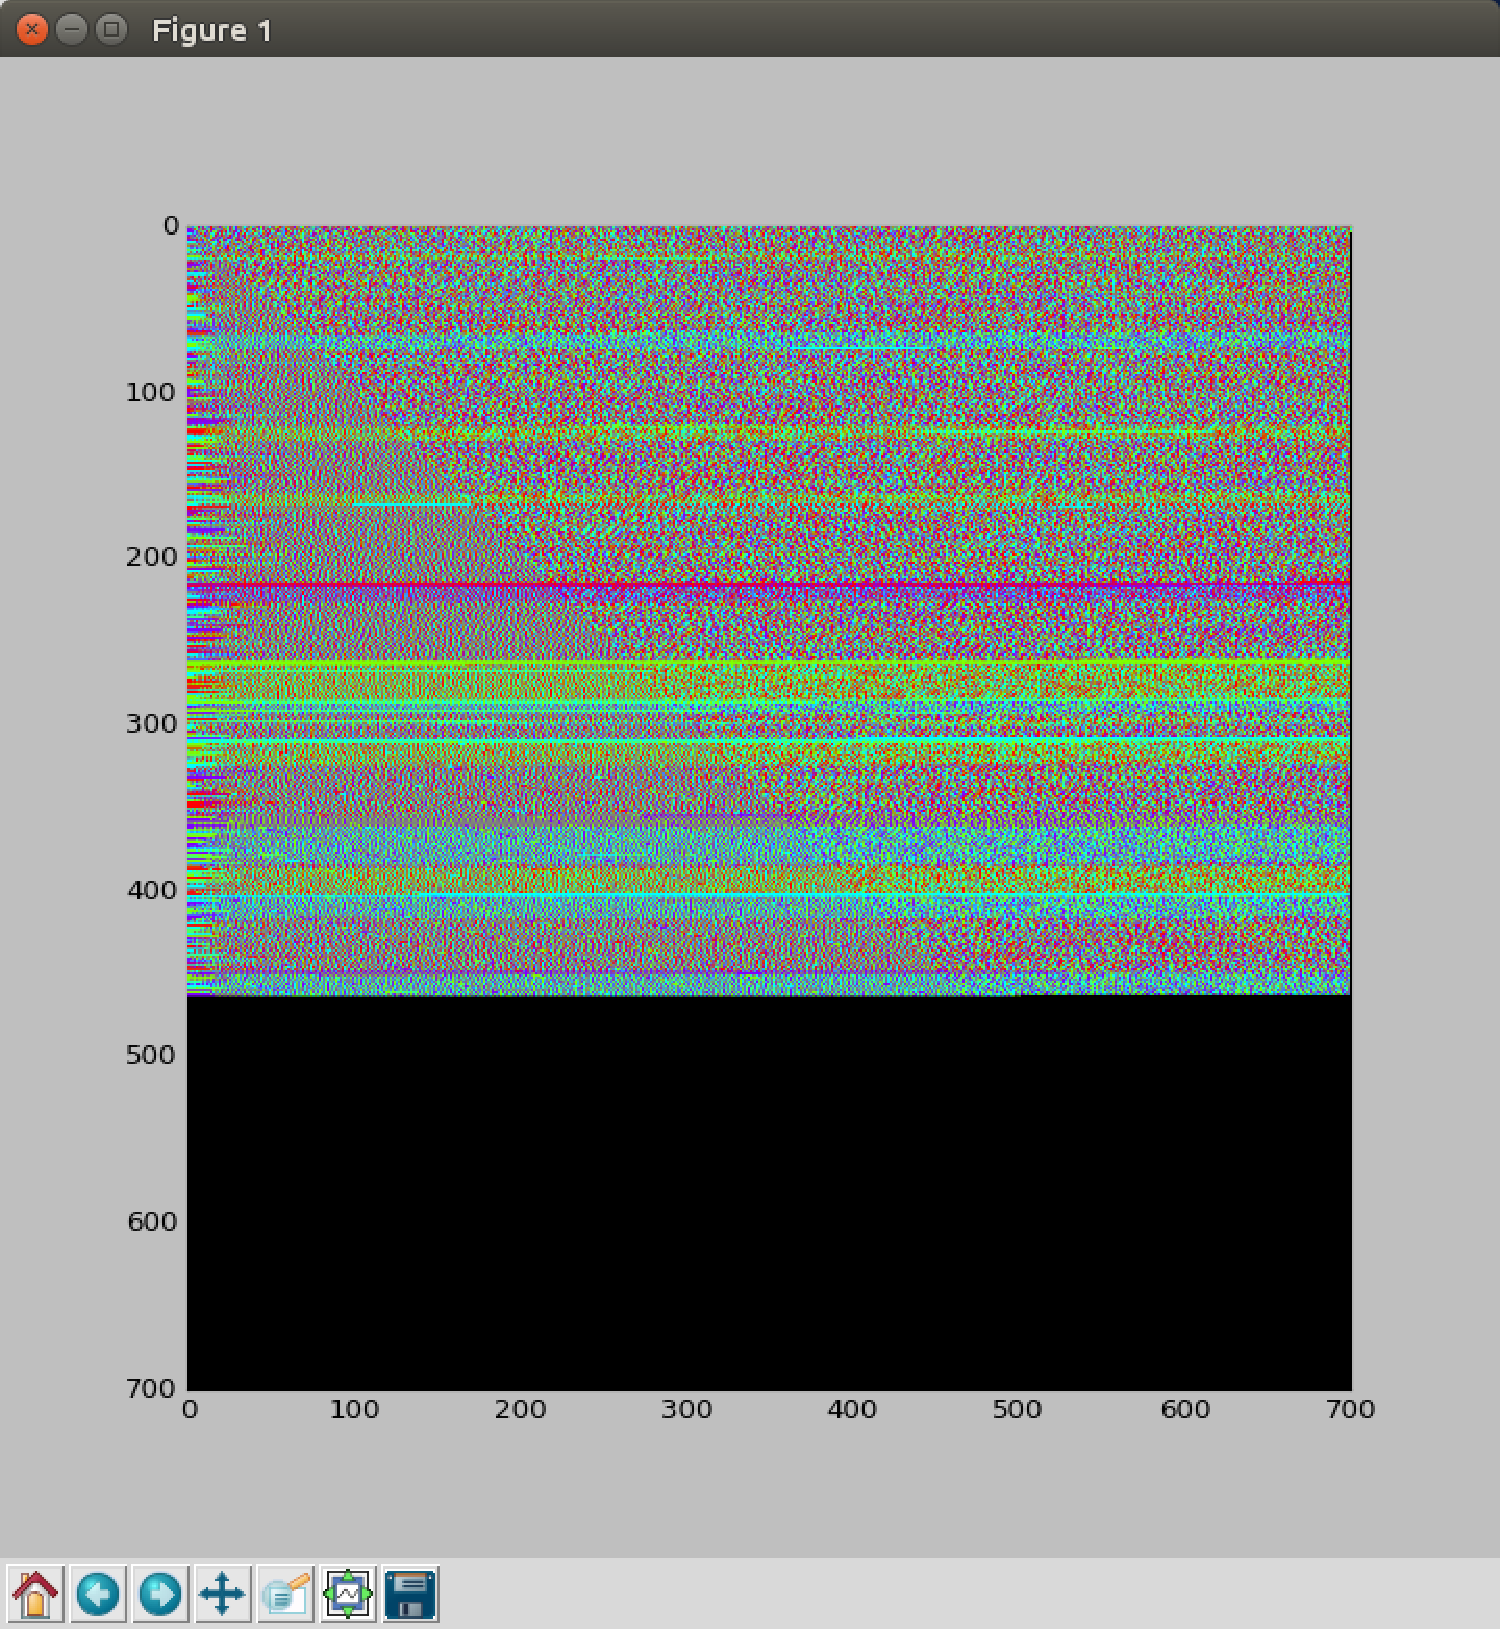
\includegraphics[width=0.8\textwidth]{out/pdf/img/load_balance_dynamic.pdf}
\vskip-2mm
{\footnotesize dynamic}
  \end{column}

  \begin{column}{0.3\textwidth}
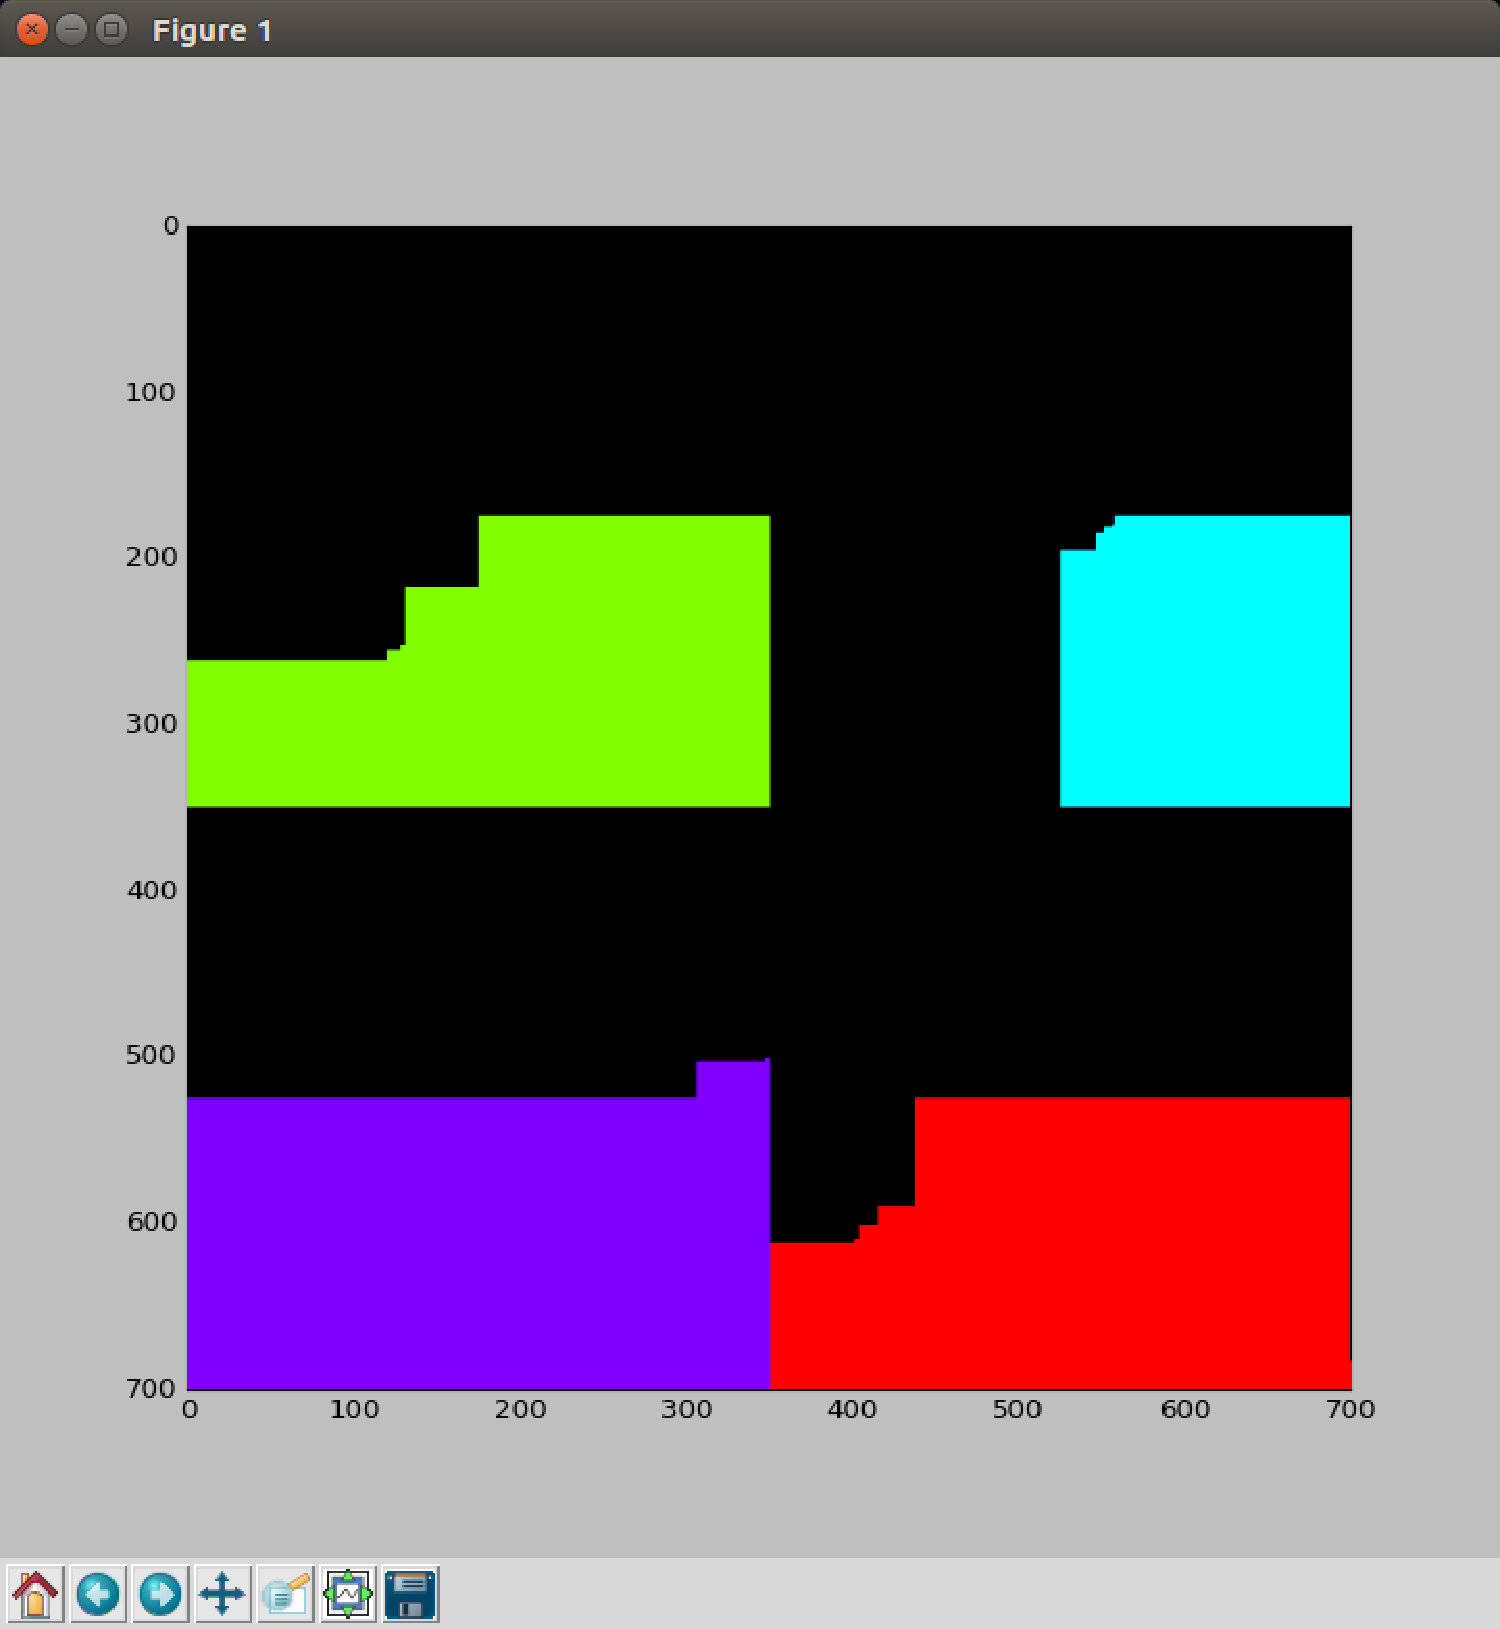
\includegraphics[width=0.8\textwidth]{out/pdf/img/load_balance_rec.pdf}
\vskip-2mm
{\footnotesize 2D recursive (midway)}

\vskip3mm
    
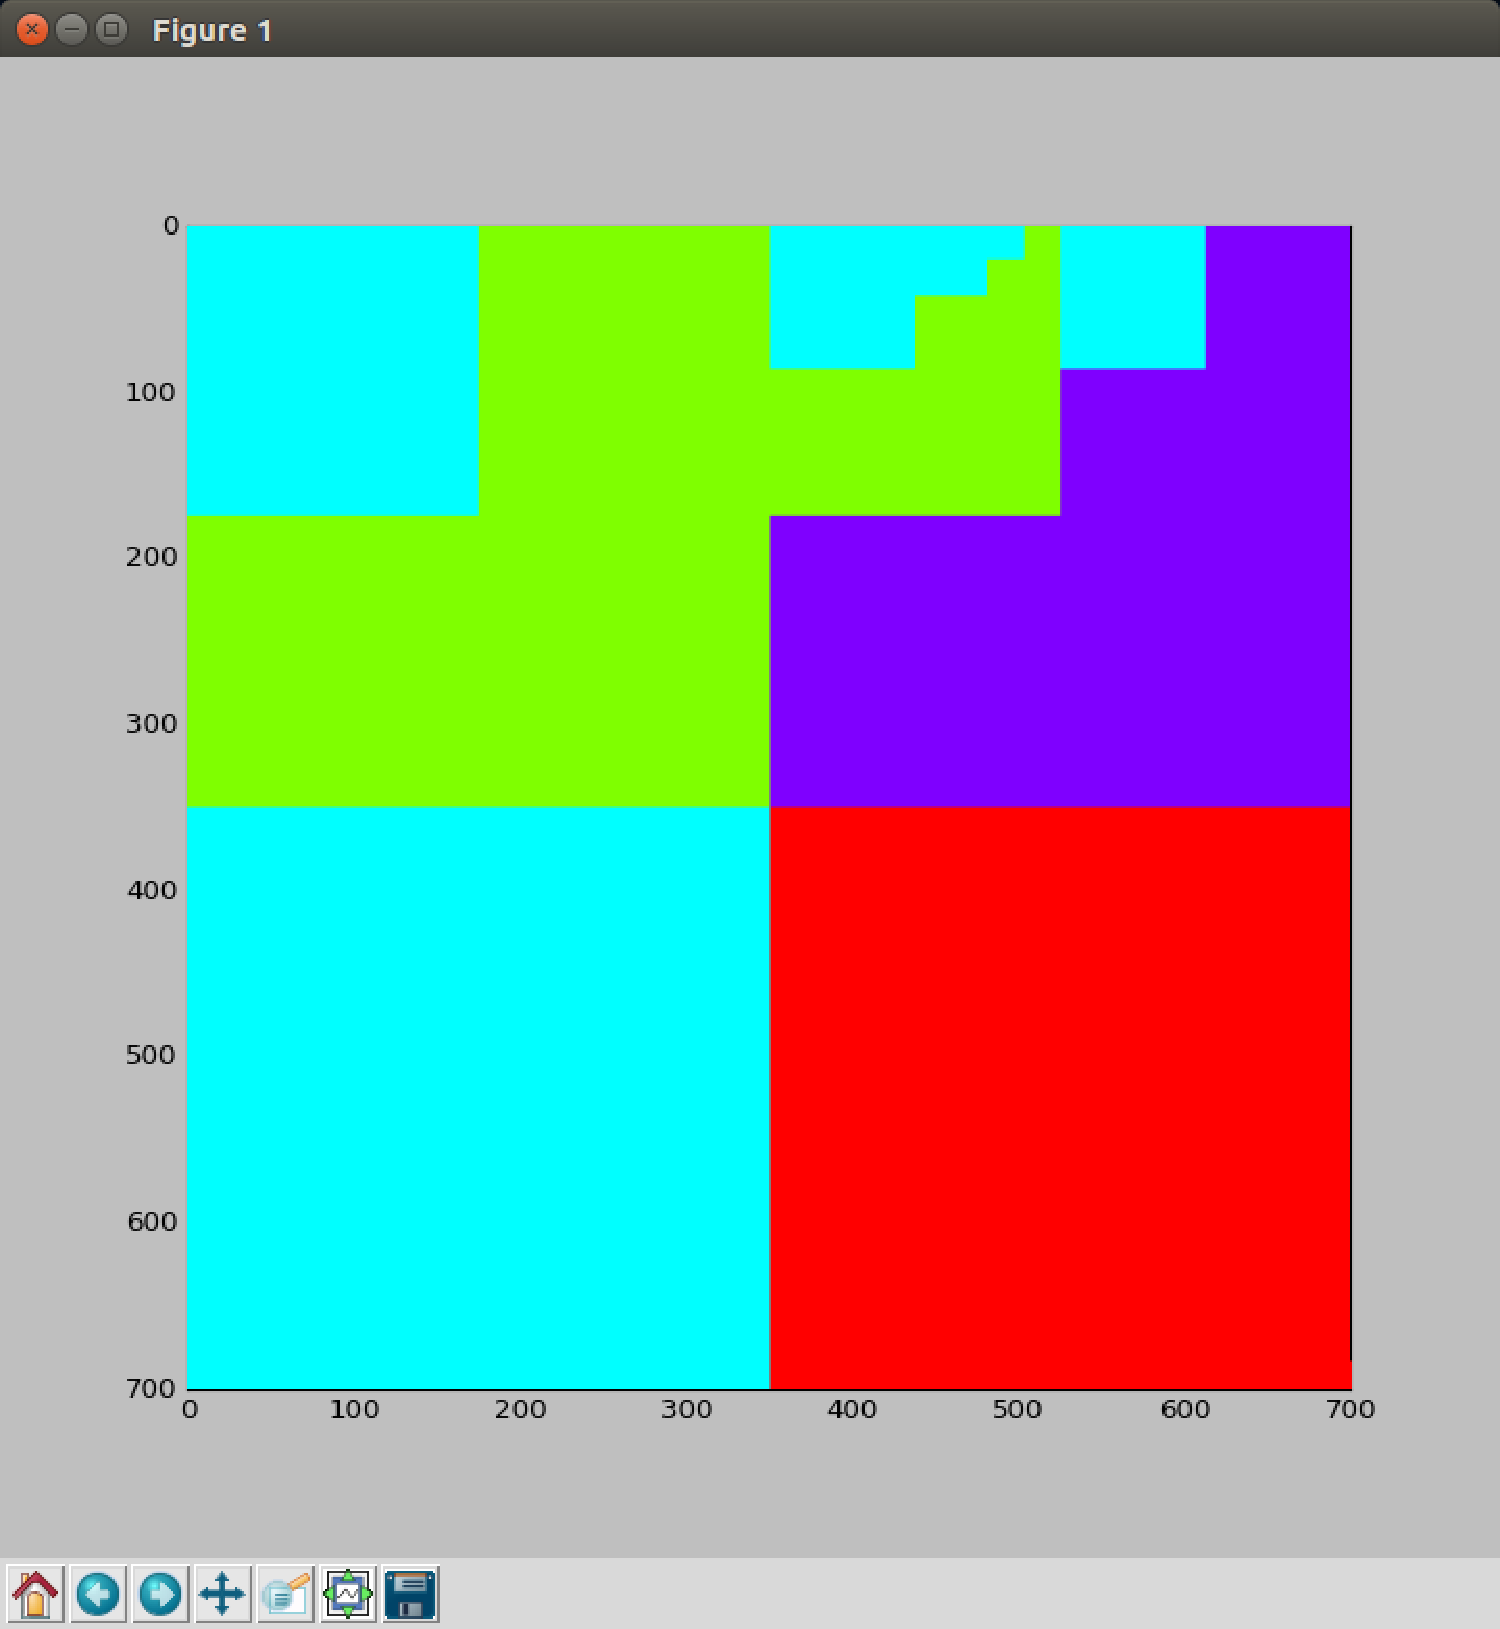
\includegraphics[width=0.8\textwidth]{out/pdf/img/load_balance_rec_end.pdf}
\vskip-2mm
{\footnotesize 2D recursive (end)}
  \end{column}

\end{columns}
\end{center}
\end{frame}

%%%%%%%%%%%%%%%%% 
\begin{frame}[fragile]
  \frametitle{SpMV with divide and conquer}
  \begin{itemize}
  \item 
    you may recursively divide the matrix $A$ submatrices, until
    nnz in a submatrix becomes sufficiently small ({\it divide and conquer})
  \item putting memory management issues aside, it is:
\begin{lstlisting}
void SpMV_rec(A, x) {
  if (nnz(A) is small) {
    return SpMV_serial(A, x, y);
  } else if (M >= N) {
    A0_,A1_ = divide_rows(A);
    y0 = SpMV_rec(A0_, x); 
    y1 = SpMV_rec(A1_, x); 
    return y0 ++ y1; // concatination
  } else {
    A_0,A_1 = divide_cols(A);
    x0,x1 = divide(x);
    y0 = SpMV_rec(A_0, x0); 
    y1 = SpMV_rec(A_0, x0); 
    return y0 + y1; // vector addition
  }
}
\end{lstlisting}
\end{itemize}
\end{frame}

%%%%%%%%%%%%%%%%% 
\begin{frame}[fragile]
\frametitle{\ldots and there is {\tt taskloop}}

\begin{itemize}
\item syntax:
\begin{lstlisting}
#pragma omp taskloop
for(i = @{\em init}@; i < @{\em limit}@; i += @{\em incr}@) 
  @$S$@
\end{lstlisting}
\item syntactic restrictions are equivalent to work-sharing for
\item conceptually, it creates tasks each of which is
  responsible for an (or a few) iteration(s)
\item unlike work-sharing for, it is generating tasks, so
  {\tt \#pragma omp taskloop} is supposed to be executed by a single thread,
  like the {\tt task} construct
\end{itemize}
\end{frame}

%%%%%%%%%%%%%%%%%
\iffalse
\begin{frame}[fragile]
\frametitle{A note on current GCC task implementation}
\begin{itemize}
\item the overhead seems high and the scalability seems low,
  so it's not very useful now
\item a pure implementation issue; nothing wrong with language spec
\item {\tt taskloop} seems even worse
\item TBB and Cilk are much better
\item Intel implementation of OpenMP tasks is good too
\item we'll come back to the topic of efficient implementation
  of task parallelism later
\end{itemize}
\end{frame}
\fi

%%%%%%%%%%%%%%%%% 
\begin{frame}[fragile]
\frametitle{Pros/cons of various approaches}
\begin{itemize}
\item {\tt static:}
  \begin{itemize}
  \item partitioning iterations is \ao{simple and does not require communication}
  \item mapping between work $\leftrightarrow$ thread is
    \ao{deterministic and predictable} (why it's important?)
  \item may cause \aka{load imbalance} (leave some threads idle,
    even when other threads have many work to do)
  \end{itemize}

\item {\tt dynamic:}
  \begin{itemize}
  \item \ao{less prone to load imbalance},
    if chunks are sufficiently small

  \item partitioning iterations \aka{needs
    communication} (no two threads execute the same
    iteration) and may become a bottleneck

  \item mapping between iterations and threads is
    \aka{non-deterministic}

  \item OpenMP's dynamic scheduler is \aka{inflexible
    in partitioning nested loops}
  \end{itemize}
\end{itemize}
\end{frame}


%%%%%%%%%%%%%%%%% 
\begin{frame}[fragile]
\frametitle{Pros/cons of schedulers}
\begin{itemize}
\item divide and conquer $+$ tasks :
  \begin{itemize}
  \item \ao{less prone to load imbalance}, as in dynamic

  \item distributing tasks \aka{needs communication, but efficient implementation techniques are known}

  \item mapping between work and thread is
    \aka{non-deterministic}, as in dynamic

  \item you can \aka{flexibly partition loop nests} in
    various ways (e.g., keep the space to square-like)

  \item need some \aka{coding efforts}
    (easily circumvented by additional libraries; 
    e.g., TBB's {\tt blocked\_range2d} and {\tt parallel\_for})

  \end{itemize}
\end{itemize}
\end{frame}


%%%%%%%%%%%%%%%%% 
\begin{frame}[fragile]
\frametitle{Deterministic and predictable schedulers}
\begin{columns}
\begin{column}{0.7\textwidth}
\begin{itemize}
\item programs often execute the same for loops many times,
  with the same trip counts, and with the same iteration
  touching a similar region 
\item such \ao{\em iterative} applications may benefit from
  reusing data brought into cache in the previous execution
  of the same loop
\item a deterministic scheduler achieves this benefit
\end{itemize}
\end{column}

\begin{column}{0.3\textwidth}
\def\svgwidth{0.6\textwidth}
{\scriptsize \input{out/tex/svg/deterministic_schedule.pdf_tex}}
\end{column}
\end{columns}

\end{frame}


%=================================
\section{Data sharing clauses}
%=================================

\begin{frame}
\frametitle{Data sharing}
\begin{itemize}
\item {\tt parallel}, {\tt for}, {\tt task} pragma accept
  clauses specifying which variables should be shared among threads
  or between the parent/child tasks
  (or otherwise privatized/replicated to each thread)
\item \sectionompdataenv\ ``Data Environments''
  \begin{itemize}
  \item \ao{\tt private}
  \item {\tt firstprivate}
  \item \ao{\tt shared}
  \item \ao{\tt reduction} (only for {\tt parallel} and {\tt for})
  \item {\tt copyin}
  % \item parallel: 
  % \item for: {\tt private, firstprivate, lastprivate, reduction}
  % \item task: {\tt private, firstprivate, shared}
  \end{itemize}
\end{itemize}
\end{frame}

%%%%%%%%%%%%%%%%% 
\begin{frame}[fragile]
\frametitle{Data sharing/privatizing example}
\begin{itemize}
\item []
\begin{lstlisting}
int main() {
  int @\mura{S}@;  /* shared */
  int @\ao{P}@;  /* made private below */
#pragma omp parallel @\ao{private(P)}@ @\mura{shared(S)}@
  {
    int @\ao{L}@; /* automatically private */
    printf("S at %p, P at %p, L at %p\n", 
           @\mura{\&S}@, @\ao{\&P}@, @\ao{\&L}@);
  }
  return 0;
}
\end{lstlisting}
\item []

{\small
\begin{lstlisting}
$ OMP_NUM_THREADS=2 ./a.out 
S at @\mura{0x..777f494}@, P at @\ao{0x..80d0e28}@, L at @\ao{0x..80d0e2c}@
S at @\mura{0x..777f494}@, P at @\ao{0x..777f468}@, L at @\ao{0x..777f46c}@
\end{lstlisting}}
% $
\end{itemize}

\end{frame}

%%%%%%%%%%%%%%%%% 
\begin{frame}[fragile]
\frametitle{Data sharing behavior}
\begin{columns}[t]
\begin{column}{0.5\textwidth}
  \begin{itemize}
  \item [] shared
  \end{itemize}
\begin{center}
\def\svgwidth{0.5\textwidth}
{\scriptsize \input{out/tex/svg/datashare.pdf_tex}}
\end{center}

  \begin{itemize}
  \item [] private
  \end{itemize}
\begin{center}
\def\svgwidth{0.5\textwidth}
{\scriptsize \input{out/tex/svg/dataprivate.pdf_tex}}
\end{center}
\end{column}

\begin{column}{0.5\textwidth}
\begin{itemize}
\item [] firstprivate
\end{itemize}
\begin{center}
\def\svgwidth{0.5\textwidth}
{\scriptsize \input{out/tex/svg/datafirstprivate.pdf_tex}}
\end{center}

\begin{itemize}
\item [] reduction
\end{itemize}
\begin{center}
\def\svgwidth{0.5\textwidth}
{\scriptsize \input{out/tex/svg/datareduction.pdf_tex}}
\end{center}
\end{column}
\end{columns}
\end{frame}

%%%%%%%%%%%%%%%%%
\iffalse
\begin{frame}[fragile]
  \frametitle{Race condition}
  \begin{itemize}
  \item \ao{definition:} there is \ao{\it a race condition}
    when concurrent threads access the same location
    and one of which writes to it
  \item \ao{\it a race condition} $\approx$
    your program won't work
  \item remember this (some accumulations may be lost)?
\begin{lstlisting}
// assume inside @\ao{\tt \#pragma omp parallel}@
   ...
@\aka{\tt \#pragma omp for}@
for (k = 0; k < A.nnz; k++) {
  i,j,Aij = A.elems[k];
  @\aka{\tt y[i]}@ += Aij * x[j];
}
\end{lstlisting}
\end{itemize}
\end{frame}
\fi

\begin{frame}[fragile]
  \frametitle{Race condition}
  \begin{itemize}
  \item \ao{definition:} there is \ao{\it a race condition}
    when concurrent threads access the same location
    and one of which writes to it
  \item \ao{\it a race condition} almost always implies
    your program won't work
  \item even something as simple as this (some accumulations may be lost)
\begin{lstlisting}
x = 123;      
#pragma omp parallel // assume we have 5 threads
{
  ...
  x++;
  ..
}
printf("x = %d\n", x)
\end{lstlisting}
\end{itemize}
\end{frame}

\begin{frame}
  \frametitle{Race condition}

  \begin{center}
  \begin{tabular}{|l|l|}
    thread 1                & thread 2                \\\hline
    x (123) $\rightarrow$ t &                         \\
                            & \only<1>{\phantom{x (123) $\rightarrow$ t}}\only<2->{x (123) $\rightarrow$ t} \\
    x $\leftarrow$ 124      &                         \\
                            & \only<2->{x $\leftarrow$ 124}      \\
  \end{tabular}
  \end{center}

  \begin{itemize}
  \item<3-> The increment by a thread is ``lost''
  \end{itemize}
\end{frame}

%%%%%%%%%%%%%%%%%
\begin{frame}
  \frametitle{Two basic tools to resolve race conditions}

  \begin{columns}
    \begin{column}{0.5\textwidth}
\begin{itemize}
\item \mura{\it ``make it atomic''}
  \ao{\tt \#pragma omp atomic} and \ao{\tt \#pragma omp critical} :
  gaurantee the specified operation to be done {\it atomically}

\item \mura{\it ``all you need may be a reduction''}
  \ao{\tt reduction} clause performs efficient {\it reduction}
  operations on behalf of you
\end{itemize}
    \end{column}
    
    \begin{column}{0.5\textwidth}
      \begin{center}{\footnotesize
        \begin{tabular}{|l|l|}
          thread 1                & thread 2                \\\hline
          x (123) $\rightarrow$ t &                         \\
          x $\leftarrow$ 124      &                         \\\hline
                                  & x (124) $\rightarrow$ t \\
                                  & x $\leftarrow$ 125      \\
        \end{tabular}}
      \end{center}
      \begin{center}
\def\svgwidth{0.5\textwidth}
{\scriptsize \input{out/tex/svg/datareduction.pdf_tex}}
\end{center}
\end{column}
\end{columns}
\end{frame}


%%%%%%%%%%%%%%%%%
\begin{frame}[fragile]
\frametitle{{\tt \#pragma omp critical}}
\begin{itemize}
\item \ao{syntax:}
\begin{lstlisting}
@\ao{\tt \#pragma omp critical}@
  @{\it statement}@
\end{lstlisting}
\item \ao{effect:} the execution of {\it statement} will not overlap
  with other executions of {\it statement} (or any other statement
  labeled {\tt \#pragma omp critical}, for that matter)
\item note: most general, but likely to be slow
\end{itemize}
\end{frame}

%%%%%%%%%%%%%%%%%
\begin{frame}[fragile]
\frametitle{{\tt \#pragma omp atomic}}
\begin{itemize}
\item \ao{syntax:}
\begin{lstlisting}
@\ao{\tt \#pragma omp atomic}@
   @{\it var}@ = @{\it var op exp}@
\end{lstlisting}
{\it op} is a predefined operation such as {\tt +, -, *, \ldots}

\item \ao{effect:} guarantee the read-update is done atomically
  (is not lost); that is,
  {\it var} is not updated by someone else
  between the read and update

\item note: semantically, it is like
\begin{lstlisting}
  @{\it e}@ = @{\it exp}@;
#pragma omp critical
  @{\it var}@ = @{\it var op e}@
\end{lstlisting}
but typical implementations take advantage of
atomic instructions supported by CPU,
such as fetch-and-add or compare-and-swap
\end{itemize}
\end{frame}

%%%%%%%%%%%%%%%%%
\begin{frame}[fragile]
\frametitle{Reduction}
\begin{columns}
\begin{column}{0.55\textwidth}
\begin{itemize}
\item in general, ``reduction'' refers to an operation to combine
  many values into a single value. e.g.,
  \begin{itemize}
  \item $v = v_1 + \cdots + v_n$
  \item $v = \max(v_1, \cdots, v_n)$
  \item \ldots
  \end{itemize}

\item simply sharing the variable ($v$) does
  not work (race condition)

\item one way to fix is to make updates atomic, but it will be slow
\end{itemize}
\end{column}

\begin{column}{0.4\textwidth}
\begin{center}
\begin{lstlisting}
@\aka{\tt v}@ = 0.0;
for (i = 0; i < n; i++) {
  @\aka{\tt v}@ += f(a + i * dt) * dt;
}    
\end{lstlisting}

\begin{lstlisting}
@\aka{\tt v}@ = 0.0;
#pragma omp parallel for
for (i = 0; i < n; i++) {
#pragma omp atomic
  @\aka{\tt v}@ += f(a + i * dt) * dt;
}    
\end{lstlisting}
\def\svgwidth{\textwidth}
{\scriptsize \input{out/tex/svg/reduction_shared.pdf_tex}}

\end{center}
\end{column}  

\end{columns}
\end{frame}


%%%%%%%%%%%%%%%%% 
\begin{frame}[fragile]
\frametitle{Reduction clause in OpenMP}
\begin{columns}
  \begin{column}{0.5\textwidth}
    \begin{itemize}
    \item a more efficient strategy:
      \begin{itemize}
      \item let each thread work (reduce) on its private variable, and
      \item when threads finish, combine their partial results into one 
      \end{itemize}

    \item {\tt reduction} clause in OpenMP does just that
      (\sectionompreduction)
\end{itemize}
\end{column}

\begin{column}{0.45\textwidth}
\begin{lstlisting}
@\ao{\tt v}@ = 0.0;
#pragma omp parallel for @\ao{\tt reduction(+:v)}@
for (i = 0; i < n; i++) {
  @\ao{\tt v}@ += f(a + i * dt) * dt;
}    
\end{lstlisting}

\def\svgwidth{\textwidth}
{\scriptsize \input{out/tex/svg/reduction.pdf_tex}}
\end{column}  

\end{columns}
\end{frame}

%%%%%%%%%%%%%%%%% 
\begin{frame}[fragile]
\frametitle{Builtin reduction and user-defined reduction (\sectionompfor)}
\begin{itemize}
\item reduction syntax:
\begin{lstlisting}
#pragma omp parallel @\ao{reduction({\em op}:{\em var,var,\ldots})}@
    @$S$@
\end{lstlisting}
\begin{itemize}
\item builtin reductions
  \begin{itemize}
  \item {\em op} is one of \verb!+, *, -, &, ^, |, &&,! and {\tt ||}
  \item (Since 3.1) {\tt min} or {\tt max}
  \end{itemize}
\item builtin reductions are \aka{\it limited to simple types and common operations}
  $\rightarrow$ \ao{\it user-defined reductions} (since 4.0) 
\end{itemize}
\end{itemize}
\end{frame}

%%%%%%%%%%%%%%%%% 
\begin{frame}[fragile]
  \frametitle{Why do you want user-defined reductions?}
  \begin{itemize}
  \item consider how to do reduction on 3-element vector
  \item e.g., how to parallelize this loop safely
\begin{lstlisting}
typedef struct {
  double a[3];
} vec_t;

int main() {
  vec_t y;
  vec_init(&y);                 /* y = {0,0,0} */
#pragma omp parallel
#pragma omp for
  for (long i = 0; i < 10000; i++) {
    @\aka{\tt y.a[i \% 3]}@ += 1;
  }
}
\end{lstlisting}
\item you cannot say \aka{\tt reduction(+:y.a[0], y.a[1], y.a[2])}
  (what if you have 100 elements?)
  
\item we define a reduction operation on {\tt vec\_t} type instead
\end{itemize}
\end{frame}

%%%%%%%%%%%%%%%%% 
\begin{frame}[fragile]
\frametitle{User-defined reduction}
\begin{itemize}
\item \ao{\tt syntax:} (\sectionompdeclarereduction)
\begin{lstlisting}
#pragma omp declare reduction (@{\em name}@ : @{\em type}@ : @{\em combine\_statement}@)
\end{lstlisting}
or
\begin{lstlisting}
#pragma omp declare reduction (@{\em name}@ : @{\em type}@ : @{\em combine\_statement}@) initializer(@{\em init\_statement}@)
\end{lstlisting}

\item \ao{effect:}
  \begin{itemize}
  \item you can specify {\tt reduction({\it name} : {\it var})}
    for a variable of type {\it type}
  \item {\it init\_statement} is executed by each thread before entering the loop, typically to initialize its private copy of {\it var}
  \item {\it combine\_statement} is executed
    to merge a partial result to another variable
  \end{itemize}
\end{itemize}
\end{frame}

%%%%%%%%%%%%%%%%% 
\begin{frame}[fragile]
\frametitle{User-defined reduction: a simple example}
\begin{itemize}
\item introduce reduction
\begin{lstlisting}
#pragma omp declare reduction \
  (@\ao{\tt vp}@ : @\ao{\tt vec\_t}@ : @\ao{\tt vec\_add(\&omp\_out,\&omp\_in)}@) \
  initializer(@\ao{\tt vec\_init(\&omp\_priv)})
\end{lstlisting}

{\tt vec\_add} must be defined somewhere and not shown

\item add {\tt reduction(vp : y)} to the for loop
\begin{lstlisting}
int main() {
  vec_t y;
  vec_init(&y);                 /* y={0,0,0} */
#pragma omp parallel
#pragma omp for @\ao{\tt reduction(vp : y)}@
  for (long i = 0; i < 10000; i++) {
    y.a[i % 3] += 1;
  }
}
\end{lstlisting}
\end{itemize}
\end{frame}

%%%%%%%%%%%%%%%%% 
\begin{frame}[fragile]
  \frametitle{User-defined reduction : how it works}
  \begin{itemize}
  \item [] with
\begin{lstlisting}
#pragma omp declare reduction \
  (@\ao{\tt vp}@ : @\ao{\tt vec\_t}@ : @\ao{\tt vec\_add(\&omp\_out,\&omp\_in)}@) \
  initializer(@\ao{\tt vec\_init(\&omp\_priv)})
\end{lstlisting}
    
  \item []
\begin{lstlisting}
#pragma omp for @\ao{\tt reduction(vp : y)}@
  for (long i = 0; i < 10000; i++) {
    y.a[i % 3] += 1;
  }
\end{lstlisting}
\item []$\approx$
\begin{lstlisting}
  @\ao{\tt vec\_t}@ y_priv; // thread-local copy of y
  @\ao{\tt vec\_init(\&y\_priv)}@; // initializer
#pragma omp for
  for (long i = 0; i < 10000; i++) {
    y_priv.a[i % 3] += 1;
  }
  // merge the partial result into the shared variable
  // actual implementation may be (is likely to be) different
  @\ao{\tt vec\_add(\&y, \&y\_priv)}@; // y += y_priv
\end{lstlisting}
\end{itemize}
\end{frame}

%%%%%%%%%%%%%%%%% 
\begin{frame}[fragile]
\frametitle{User-defined reduction : limitations}
\begin{itemize}
\item {\it combine-statement} can reference
  only two local variables (\ao{\tt omp\_in} and \ao{\tt omp\_out})
  \begin{itemize}
  \item it should reduce (merge) {\tt omp\_in} into {\tt omp\_out}
    (e.g., {\tt omp\_out += omp\_in})
  \end{itemize}
\item {\it init-statement} can reference
  only two local variables (\ao{\tt omp\_priv} and \ao{\tt omp\_orig})
  \begin{itemize}
  \item {\tt omp\_priv} : the private copy {\it init-statement}
    should initialize
  \item {\tt omp\_orig} : the original shared variable
  \end{itemize}

\item $\Rightarrow$ local contexts necessary for
  initialization and reduction must be 
  encapsulated in the variables subject to reduction
\end{itemize}
\end{frame}


%%%%%%%%%%%%%%%%% 
\begin{frame}[fragile]
\frametitle{An exercise : reduction on variable-length vectors}
\begin{itemize}
\item a variable-length version of the previous example
\begin{lstlisting}
typedef struct {
  long @\aka{\tt n}@;     // number of elements (variable)
  double * a; // n elements
} vec_t;
\end{lstlisting}

\item and a reduction for it
\begin{lstlisting}
  vec_t y;
  long n = 100;
  vec_init(&y, @\aka{\tt n}@); // n is a local context
#pragma omp parallel
#pragma omp for    // how to do a proper reduction for y?
  for (long j = 0; j < 1000000; j++) {
    y.a[j % n] += 1;
  }
\end{lstlisting}

\item the point is you cannot reference \aka{\it n} in the initializer

\begin{lstlisting}
@\aka{(!)}@ #pragma omp declare reduction \
  (@\ao{\tt vp}@ : @\ao{\tt vec\_t}@ : @\ao{\tt vec\_add(\&omp\_out,\&omp\_in)}@) \
  initializer(@\ao{\tt vec\_init(\&omp\_priv, \aka{\tt n})})
\end{lstlisting}
\end{itemize}
\end{frame}

%%%%%%%%%%%%%%%%% 
\begin{frame}[fragile]
\frametitle{An exercise : reduction on variable-length vectors}
\begin{itemize}
\item initializer can reference {\tt omp\_orig} to obtain the context
  (i.e. vector length in this example)

\item $\Rightarrow$ define a function, {\tt vec\_init\_from},
  which takes the shared {\tt y} and initialize the private copy of {\tt y}
  
\begin{lstlisting}
int vec_init_from(vec_t * v, vec_t * orig) {
  long n = orig->n;
  double * a = (double *)malloc(sizeof(double) * n);
  for (long i = 0; i < n; i++) {
    a[i] = 0;
  }
  v->n = n;
  v->a = a;
  return 0;
}
\end{lstlisting}

\item and say
\begin{lstlisting}
#pragma omp declare reduction \
  (vp : vec_t : vec_add(&omp_out,&omp_in)) \
  initializer(@\ao{\tt vec\_init\_from(\&omp\_priv, \&omp\_orig)})
\end{lstlisting}
\end{itemize}
\end{frame}

%%%%%%%%%%%%%%%%%
%=================================
\section{SIMD constructs}
%=================================

%%%%%%%%%%%%%%%%%%%%%%%%%%%%%%
\begin{frame}[fragile]
\frametitle{SIMD constructs}
\begin{itemize}
\item {\tt simd} pragma (\sectionompsimd)
  \begin{itemize}
  \item allows an explicit vectorization of for loops
  \item syntax restrictions similar to {\tt omp for} pragma apply
  \end{itemize}

\item {\tt declare simd} pragma (\sectionompdeclaresimd)
  \begin{itemize}
  \item instructs the compiler to generate vectorized versions of a function
  \item with it, loops with function calls can be vectorized
  \end{itemize}
\end{itemize}
\end{frame}

%%%%%%%%%%%%%%%%%%%%%%%%%%%%%%
\begin{frame}[fragile]
\frametitle{{\tt simd} pragma}
\begin{itemize}
\item basic syntax (similar to {\tt omp for}):
\begin{lstlisting}
#pragma omp @\ao{\tt simd}@ @{\em clauses}@
for (i = ...; i < ...; i += ...) 
    @$S$@
\end{lstlisting}

\item clauses
  \begin{itemize}
  \item {\tt aligned({\it var,var,\ldots}:{\it align})}
  \item {\tt uniform({\it var,var,\ldots})} says variables are loop invariant
  \item {\tt linear({\it var,var,\ldots}:{\it stride})} 
    says variables have the specified stride between consecutive iterations
  \end{itemize}
\end{itemize}
\end{frame}


%%%%%%%%%%%%%%%%%%%%%%%%%%%%%%
\begin{frame}[fragile]
\frametitle{{\tt declare simd} pragma}
\begin{itemize}
\item basic syntax (similar to {\tt omp for}):
\begin{lstlisting}
#pragma omp @\ao{\tt declare simd}@ @{\em clauses}@
@{\it function definition}@
\end{lstlisting}

\item clauses
  \begin{itemize}
  \item those for {\tt simd} pragma
  \item {\tt notinbranch}
  \item {\tt inbranch}
  \end{itemize}

\end{itemize}
\end{frame}

%%%%%%%%%%%%%%%%%%%%%%%%%%%%%%
\begin{frame}
\frametitle{SIMD pragmas, rationales}
\begin{itemize}
\item most automatic vectorizers give up vectorization in many cases
  \begin{enumerate}
  \item conditionals (lanes may branch differently)
  \item inner loops (lanes may have different trip counts)
  \item function calls (function bodies are not vectorized)
  \item iterations may not be independent
  \end{enumerate}

\item {\tt simd} and {\tt declare simd} directives
  should eliminate obstacles 3 and 4 and
  significantly enhance vectorization opportunities

\end{itemize}
\end{frame}

%%%%%%%%%%%%%%%%%%%%%%%%%%%%%%
\begin{frame}[fragile]
\frametitle{A note on GCC OpenMP SIMD implementation}
\begin{itemize}
\item GCC {\tt simd} and {\tt declare simd}
  $\approx$ existing auto vectorizer $-$ dependence analysis

\item {\tt declare simd} functions are first converted into a loop
  over all vector elements and then passed to the loop vectorizer

\begin{columns}
\begin{column}{0.4\textwidth}
\begin{lstlisting}
#pragma omp declare simd
float f(float x, float y) {
  return x + y;
}
\end{lstlisting}
\end{column}
\begin{column}{0.05\textwidth}
$\rightarrow$
\end{column}
\begin{column}{0.45\textwidth}
\begin{lstlisting}
float8 f(float8 vx, float8 vy) {
  float8 r;
  for (i = 0; i < 8; i++) {
    float x = vx[i], y = vy[i]
    r[i] = x + y;
  }
  return r;
}
\end{lstlisting}
\end{column}
\end{columns}


\item the range of vectorizable loops in a
  recent version I investigated (7.3.0) seems very limited
  \begin{itemize}
  \item innermost loop with no conditionals
  \item doubly nested loop with a very simple inner loop
  \end{itemize}
\end{itemize}
\end{frame}

%%%%%%%%%%%%%%%%% 
\begin{frame}
\frametitle{Strategies for SpMV}
\begin{itemize}
\item parallelize only across different rows
  (a single row is processed sequentially)
  \begin{itemize}
  \item especially natural for CSR
  \item extremely long rows may limit speedup
  \end{itemize}

\item parallelize all non-zeros, with careful handling of {\tt y[i] +=}
  \begin{itemize}
  \item atomic accumulation ({\tt \#pragma omp atomic})
  \item reduction ({\tt \#pragma omp reduction}).
    you must have user-defined reduction
  \end{itemize}

\item divide rows until the number of non-zeros becomes small
  (e.g., $\leq 5000$)
  \begin{itemize}
  \item further divide a single row if a row contains many zeros
  \item can be done naturally with tasks
  \end{itemize}
  
\end{itemize}
\end{frame}



\end{document}


%% template
\begin{frame}[fragile]
\frametitle{fragile and columns}
\begin{columns}
\begin{column}{0.5\textwidth}
  \begin{itemize}
  \item 
  \end{itemize}
\end{column}

\begin{column}{0.5\textwidth}
\begin{center}
\def\svgwidth{\textwidth}
%{\scriptsize \input{out/tex/svg/xxxxxx.pdf_tex}}
\end{center}
\end{column}
\end{columns}
\end{frame}
